\documentclass[11pt,xcolor=dvipsnames]{beamer}
\usetheme{nelle}
\usepackage{natbib}                 % Fancy bibliography.
\usepackage{url}                    % Allow printing of URLs.
\usepackage{outlines}
\usepackage{enumitem}
\usepackage{multicol}
\usepackage{dsfont}
\usepackage{amsmath}
\usepackage{epstopdf}
\usepackage{color}
\usepackage[utf8]{inputenc}
\usepackage{tikz}
\usetikzlibrary{decorations.pathreplacing,positioning, arrows.meta}

\setbeamerfont{caption}{size=\scriptsize}
\setbeamertemplate{navigation symbols}{}
\setbeamertemplate{footline}{%
\hfill\usebeamertemplate***{navigation symbols}
\raisebox{2pt}[0pt][0pt]{%
\color{gray}\hspace{1cm} \insertframenumber{} }
}

\def\newblock{\hskip .11em plus .33em minus .07em}

\title{\textbf{Apprentissage statistique en haute dimension}\\
{\large Structures, fonctions et régulation des génomes.}}
\subtitle{Candidature CR-CN en Section 07 au LIRIS (UMR 5205)}
\author[Varoquaux Nelle]{%
Nelle Varoquaux}
\date{28 Mars, 2019}
\institute{Department of Statistics, University of California, Berkeley}

\begin{document}
\begin{frame}[t, noframenumbering]
  \maketitle
\end{frame}

\setcounter{framenumber}{0}


\begin{frame}
\frametitle{Nelle Varoquaux}

\begin{columns}
\begin{column}{0.8\linewidth}
{\bf \footnotesize Un parcours entre l'informatique, les statistiques et la
biologie}
\vskip-1.3ex
\rule{\dimexpr\paperwidth-2.5cm\relax}{0.4pt}
\begin{itemize}[leftmargin=*]
\scriptsize
\item[-] 2010 Ingénieur {\bf Centrale Nantes} (spécialité info)
\item[-] 2010-2011 Ingénieur logiciel R\&D The pH Group, à Londres
\item[-] 2011-2012 M2 Mathématiques appliquées, Vision et Apprentissage à l'{\bf ENS Cachan}
\item[-] 2012-2015 Thèse à {\bf Mines ParisTech}, équipe CBIO
\begin{itemize}
    \scriptsize
    \item[-] {\bf Développement de méthodes statistiques pour l'analyse de la
    structure 3D du génome}
\end{itemize}
\item[-] 2016-2019 Postdoctorat à {\bf UC Berkeley}, département de
statistiques
\begin{itemize}
    \scriptsize
    \item[-] {\bf Analyse fonctionnelle pour l'étude de
    données longitudinales}
\end{itemize}
\end{itemize}

\begin{overlayarea}{10cm}{4cm}
\only<2->{%
{\bf \scriptsize Bourses \& distinctions}
\vskip-1.3ex
\rule{\dimexpr\paperwidth-3cm\relax}{0.4pt}
\begin{itemize}[leftmargin=*]
    \scriptsize
    \item[-] Moore-Sloan data science fellow à BIDS\quad {\tiny (5\% des candidats
    sélectionnés)}
    \item[-] EMBER\quad Exploring maintainer burnout with ethnographic
    research\quad {\tiny (\$138 035) }
\end{itemize}

}
\only<3->{%
{\bf \scriptsize Implications scientifiques}
\vskip-1.3ex
\rule{\dimexpr\paperwidth-3cm\relax}{0.4pt}
\begin{itemize}[leftmargin=*]
\scriptsize
\item[-] Grands consortiums {\tiny ({\em e.g} \quad \textbf{EPICON}\quad EPIgenetic CONtrol of
drought resistance in sorghum)}
\item[-] Organisation de congrès, conférences \& écoles d'été {\tiny (GraphXD, SciPy,
EuroScipy, ASPP \dots)}
\end{itemize}

\includegraphics[width=0.15\linewidth]{images/matplotlib.png} \quad

\includegraphics[width=0.12\linewidth]{images/scikit-learn.png} \quad

\includegraphics[width=0.15\linewidth]{images/scikit-image.png}
}
\end{overlayarea}


\end{column}
\begin{column}{0.08\linewidth}

\includegraphics[width=0.9\linewidth]{images/centrale_nantes.png} \\
\vspace{15pt}

\includegraphics[width=0.9\linewidth]{images/ens_cachan.png} \\
\vspace{15pt}

\includegraphics[width=0.9\linewidth]{images/ecole_des_mines.png} \\
\vspace{15pt}

\includegraphics[width=0.9\linewidth]{images/uc_berkeley.png} \\
\vspace{15pt}

\includegraphics[width=0.9\linewidth]{images/bids.png} \\
\vspace{15pt}

\includegraphics[width=0.9\linewidth]{images/moore_foundation.jpg} \\
\vspace{15pt}

\includegraphics[width=0.9\linewidth]{images/sloan_foundation.png}
\end{column}
\end{columns}

\end{frame}

\begin{frame}
\frametitle{La régulation des gènes et l'épigénétique}
\vspace{-0.5em}
\begin{figure}
\centering
\only<1-2>{%
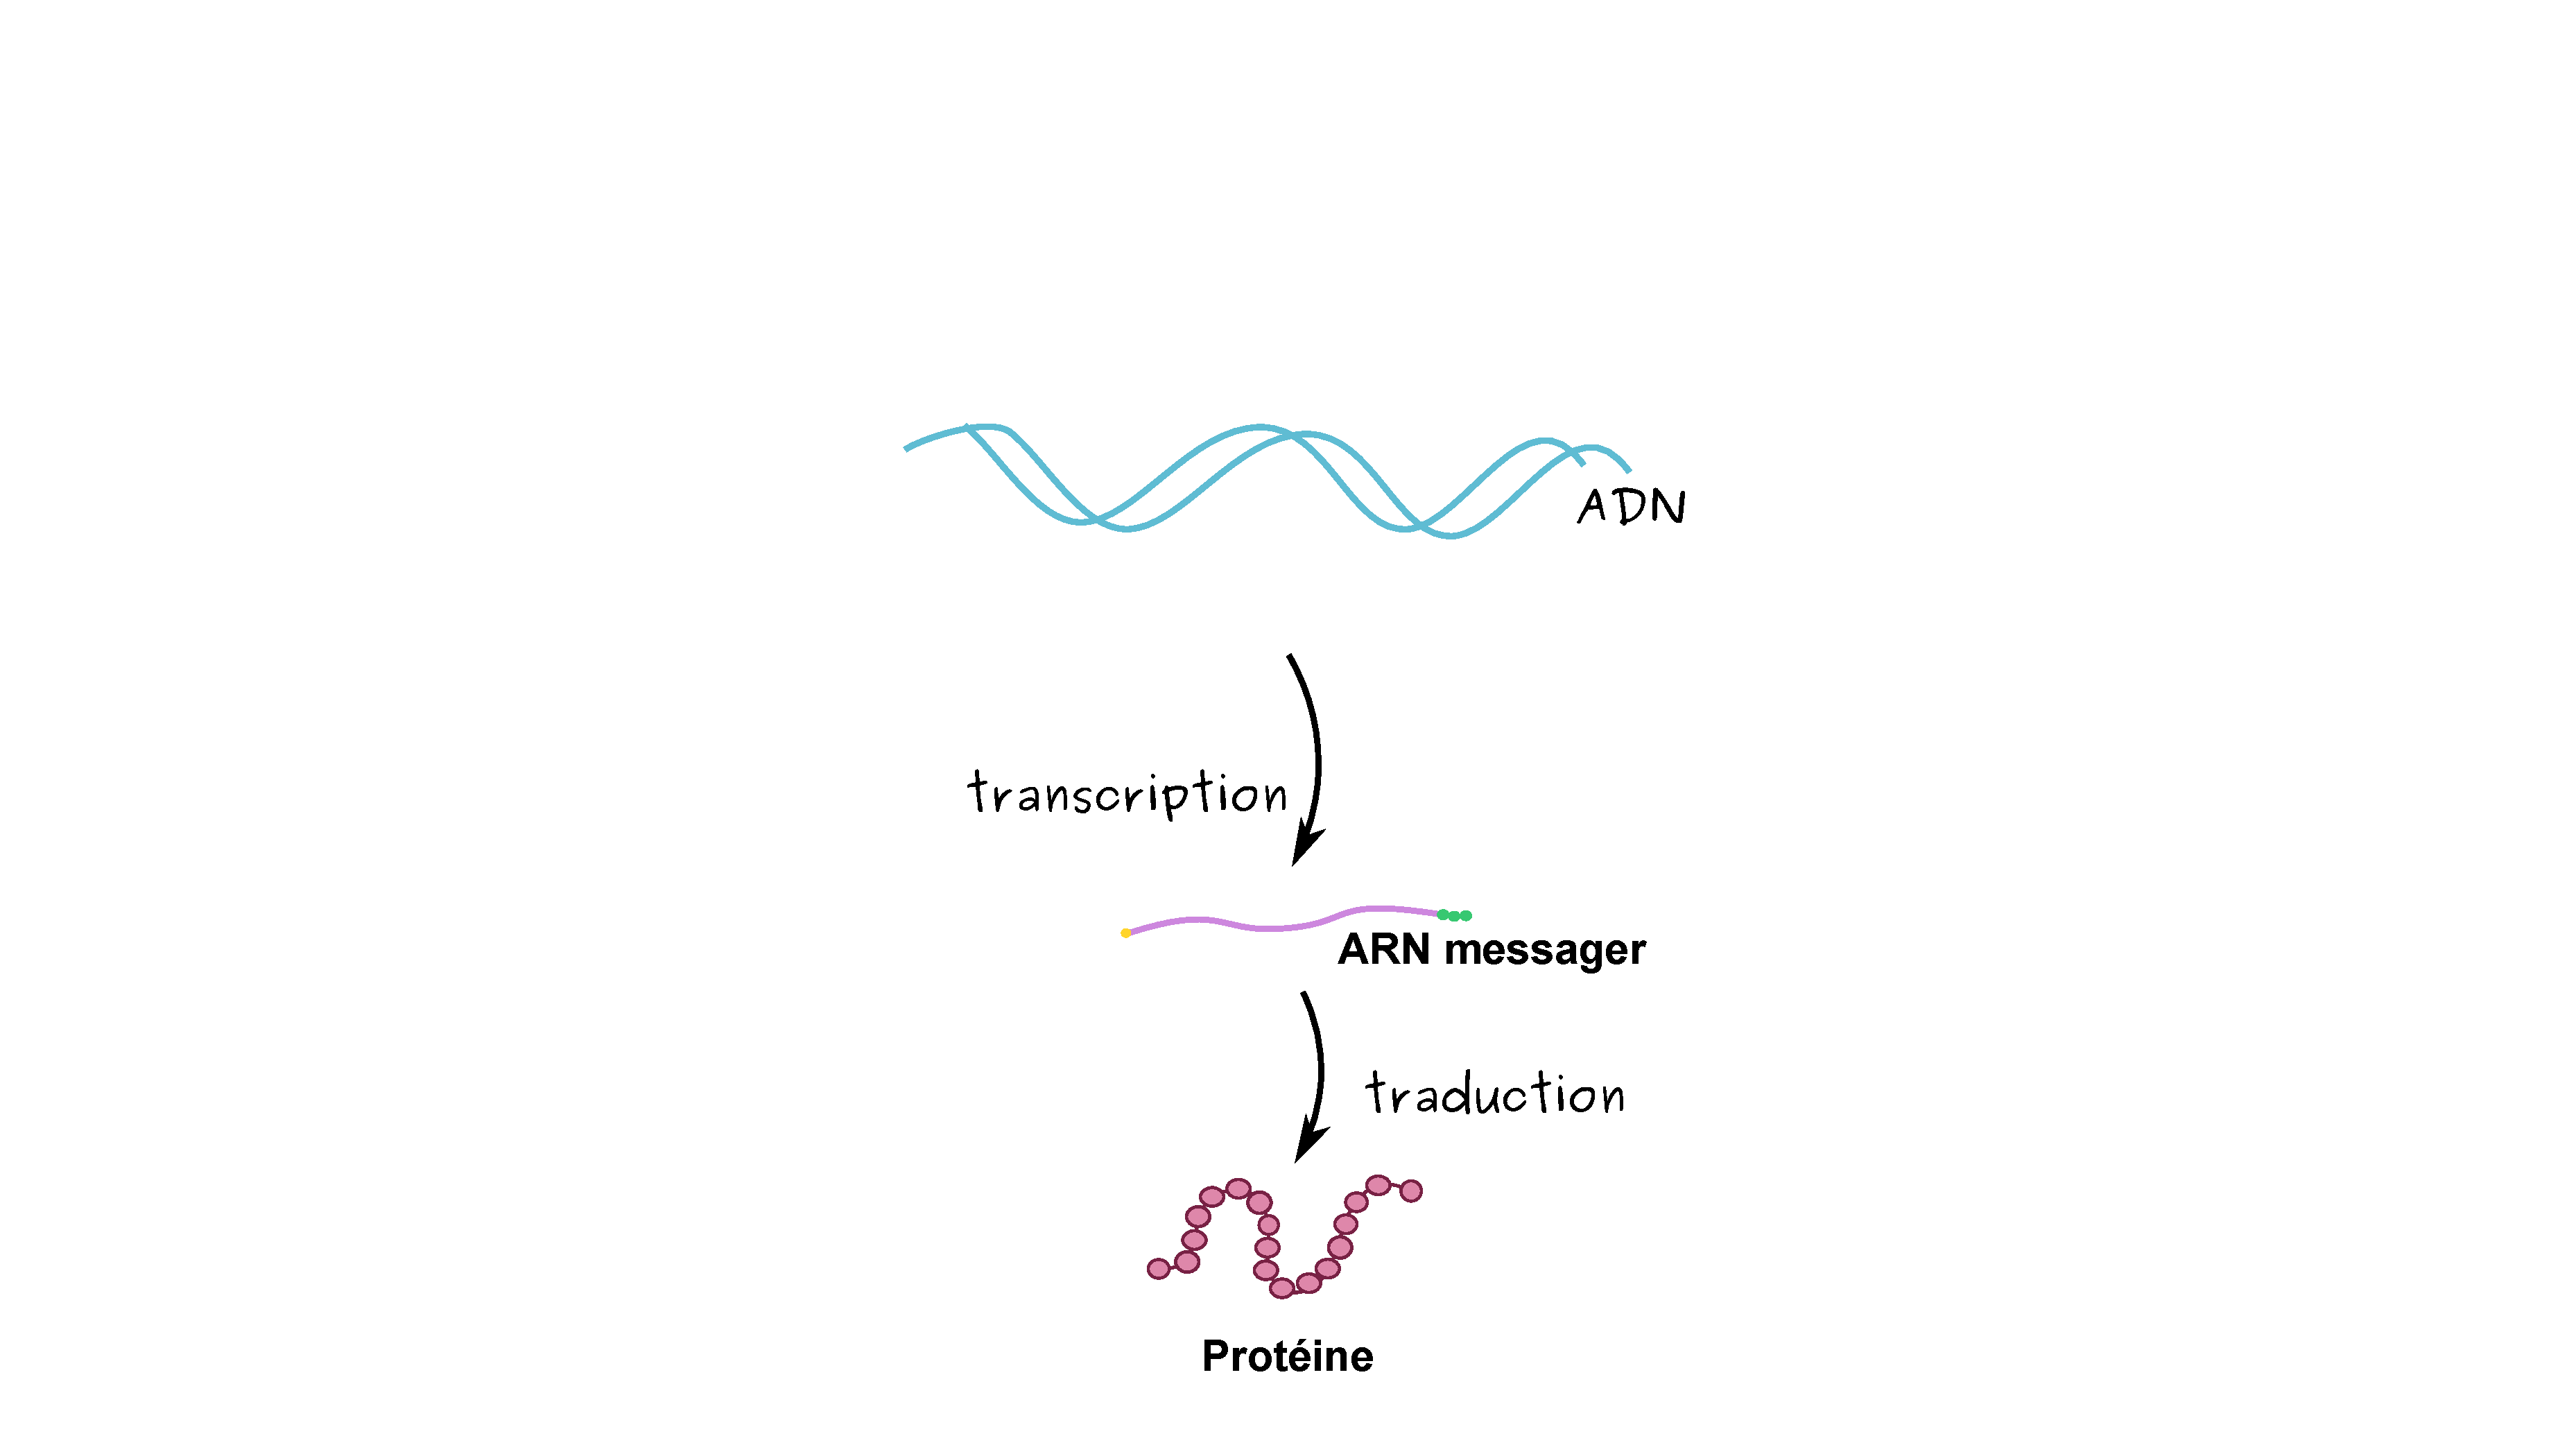
\includegraphics[width=0.9\linewidth]{schemas/gene_regulation_final_1.pdf}}%
\only<3>{%
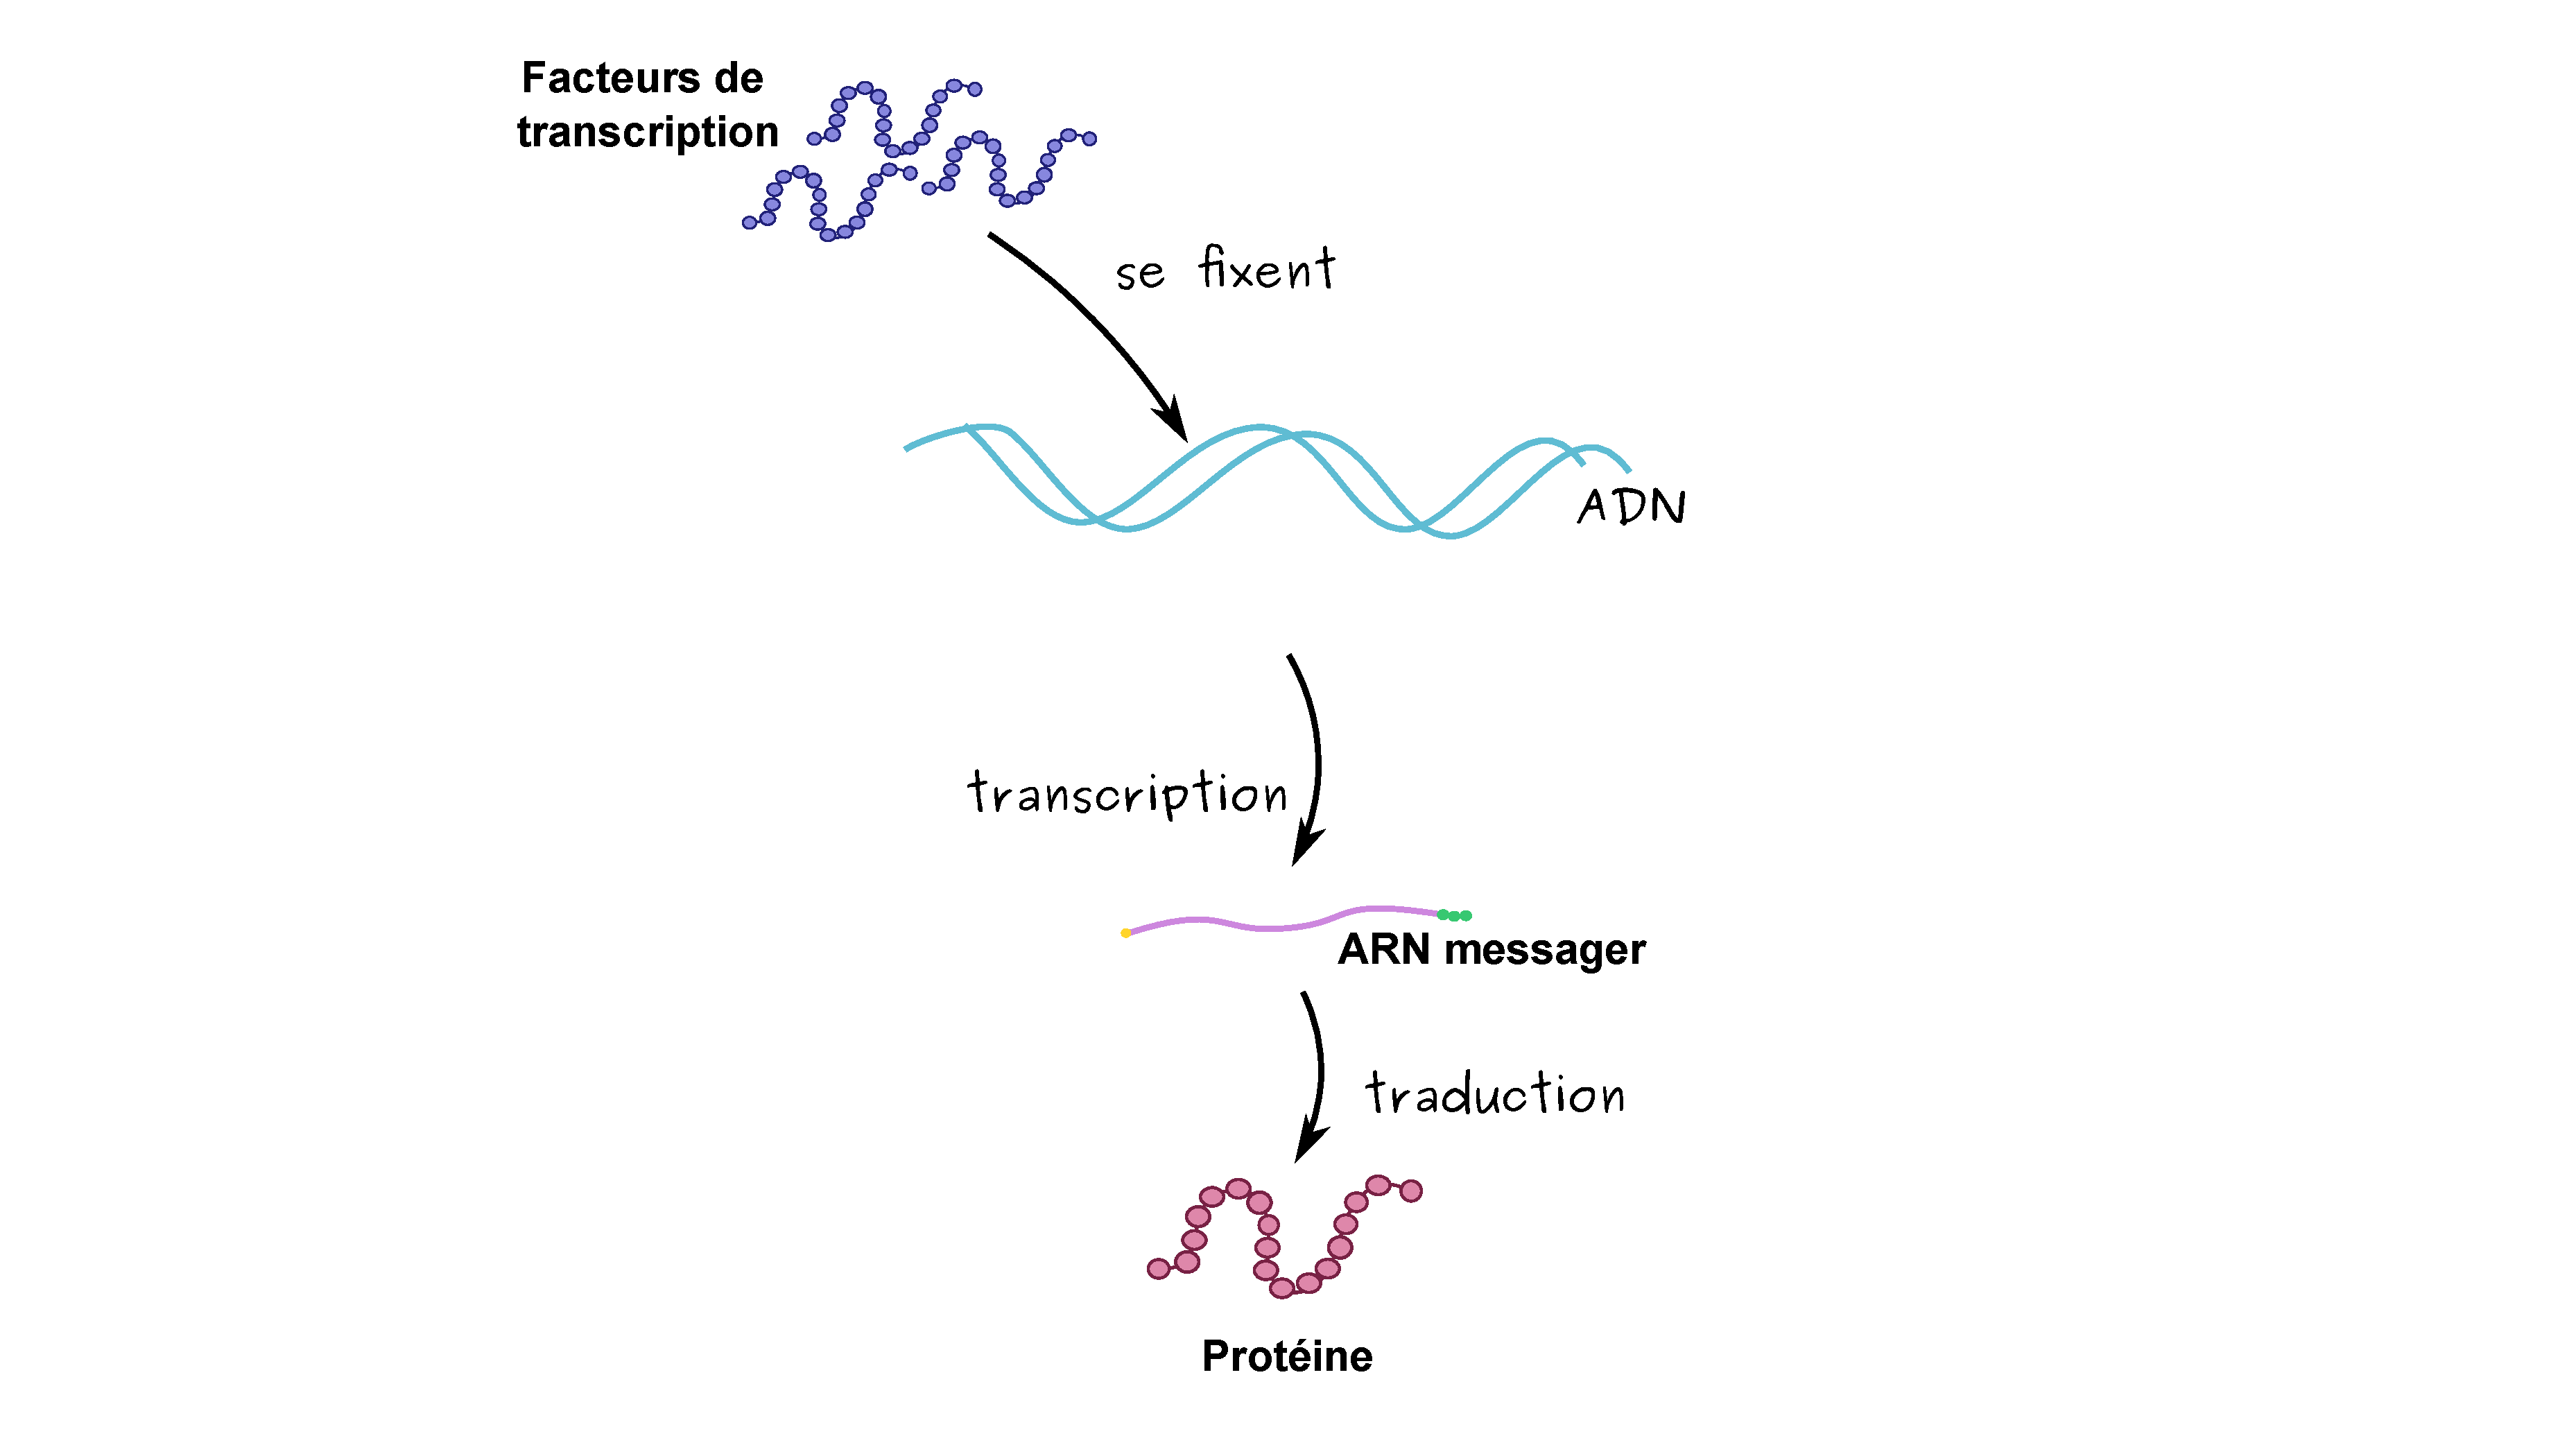
\includegraphics[width=0.9\linewidth]{schemas/gene_regulation_final_2.pdf}}%
\only<4>{%
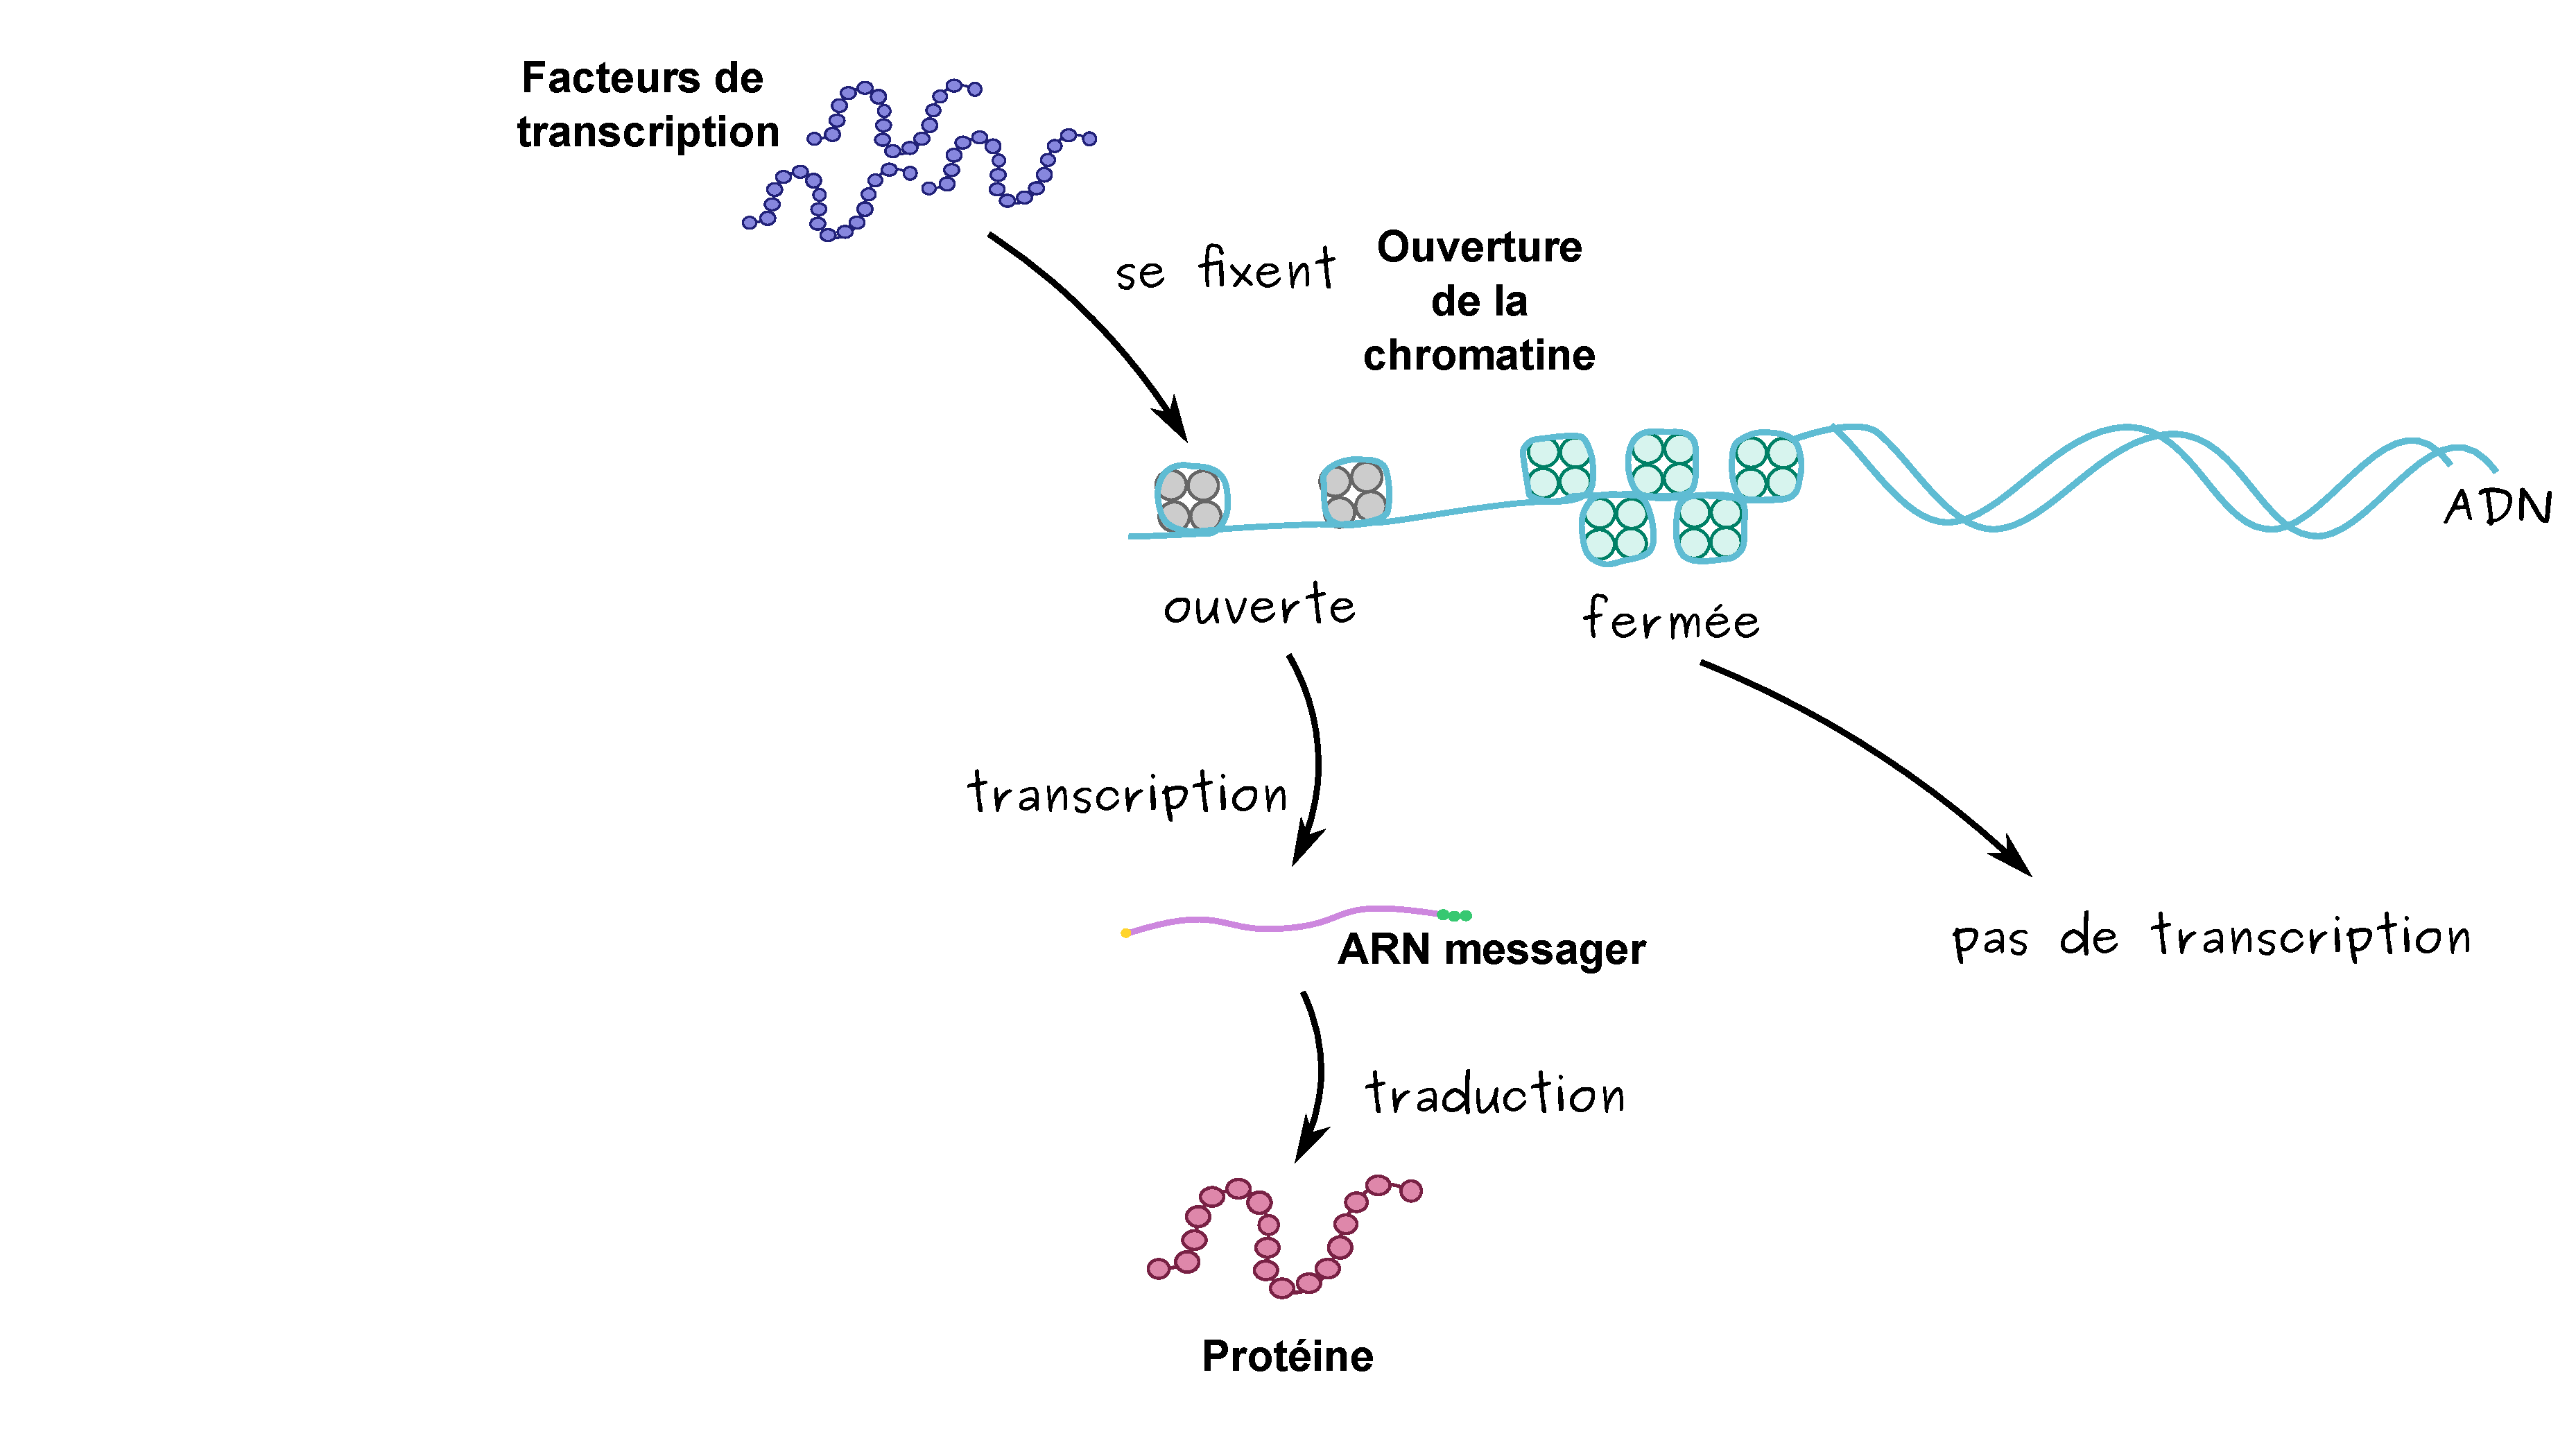
\includegraphics[width=0.9\linewidth]{schemas/gene_regulation_final_3.pdf}}%
\only<5>{%
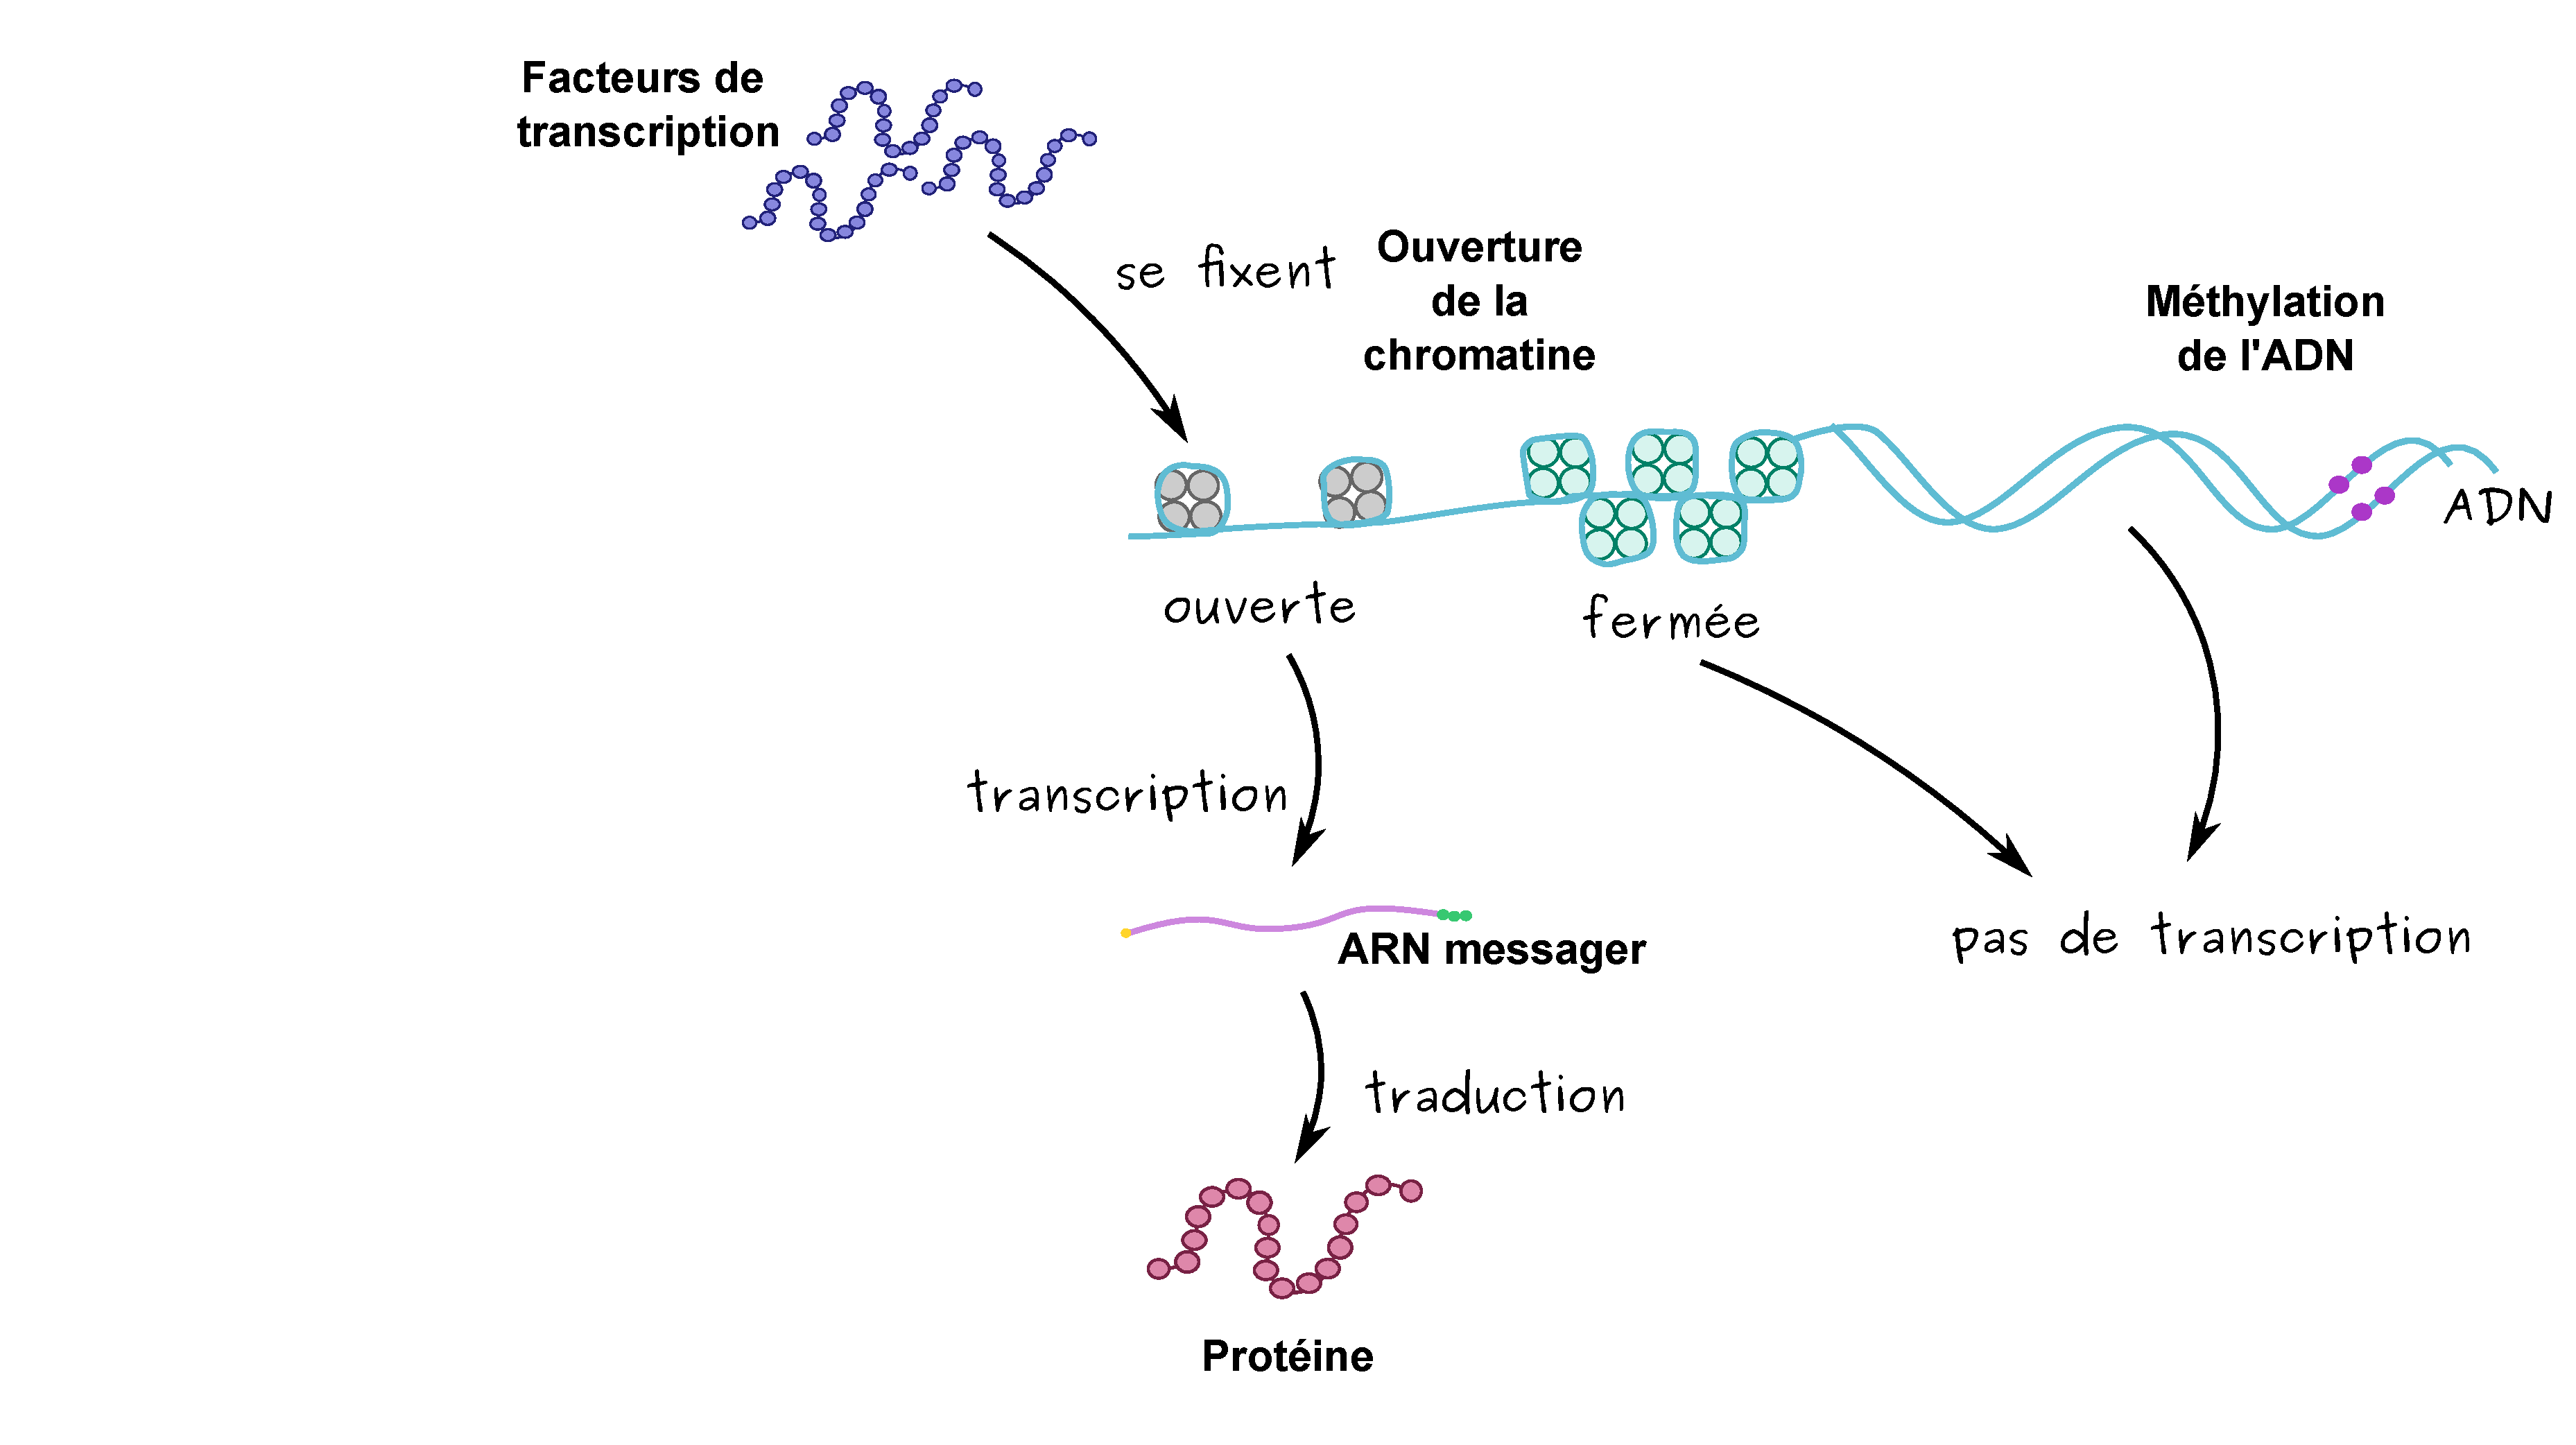
\includegraphics[width=0.9\linewidth]{schemas/gene_regulation_final_4.pdf}}%
\only<6>{%
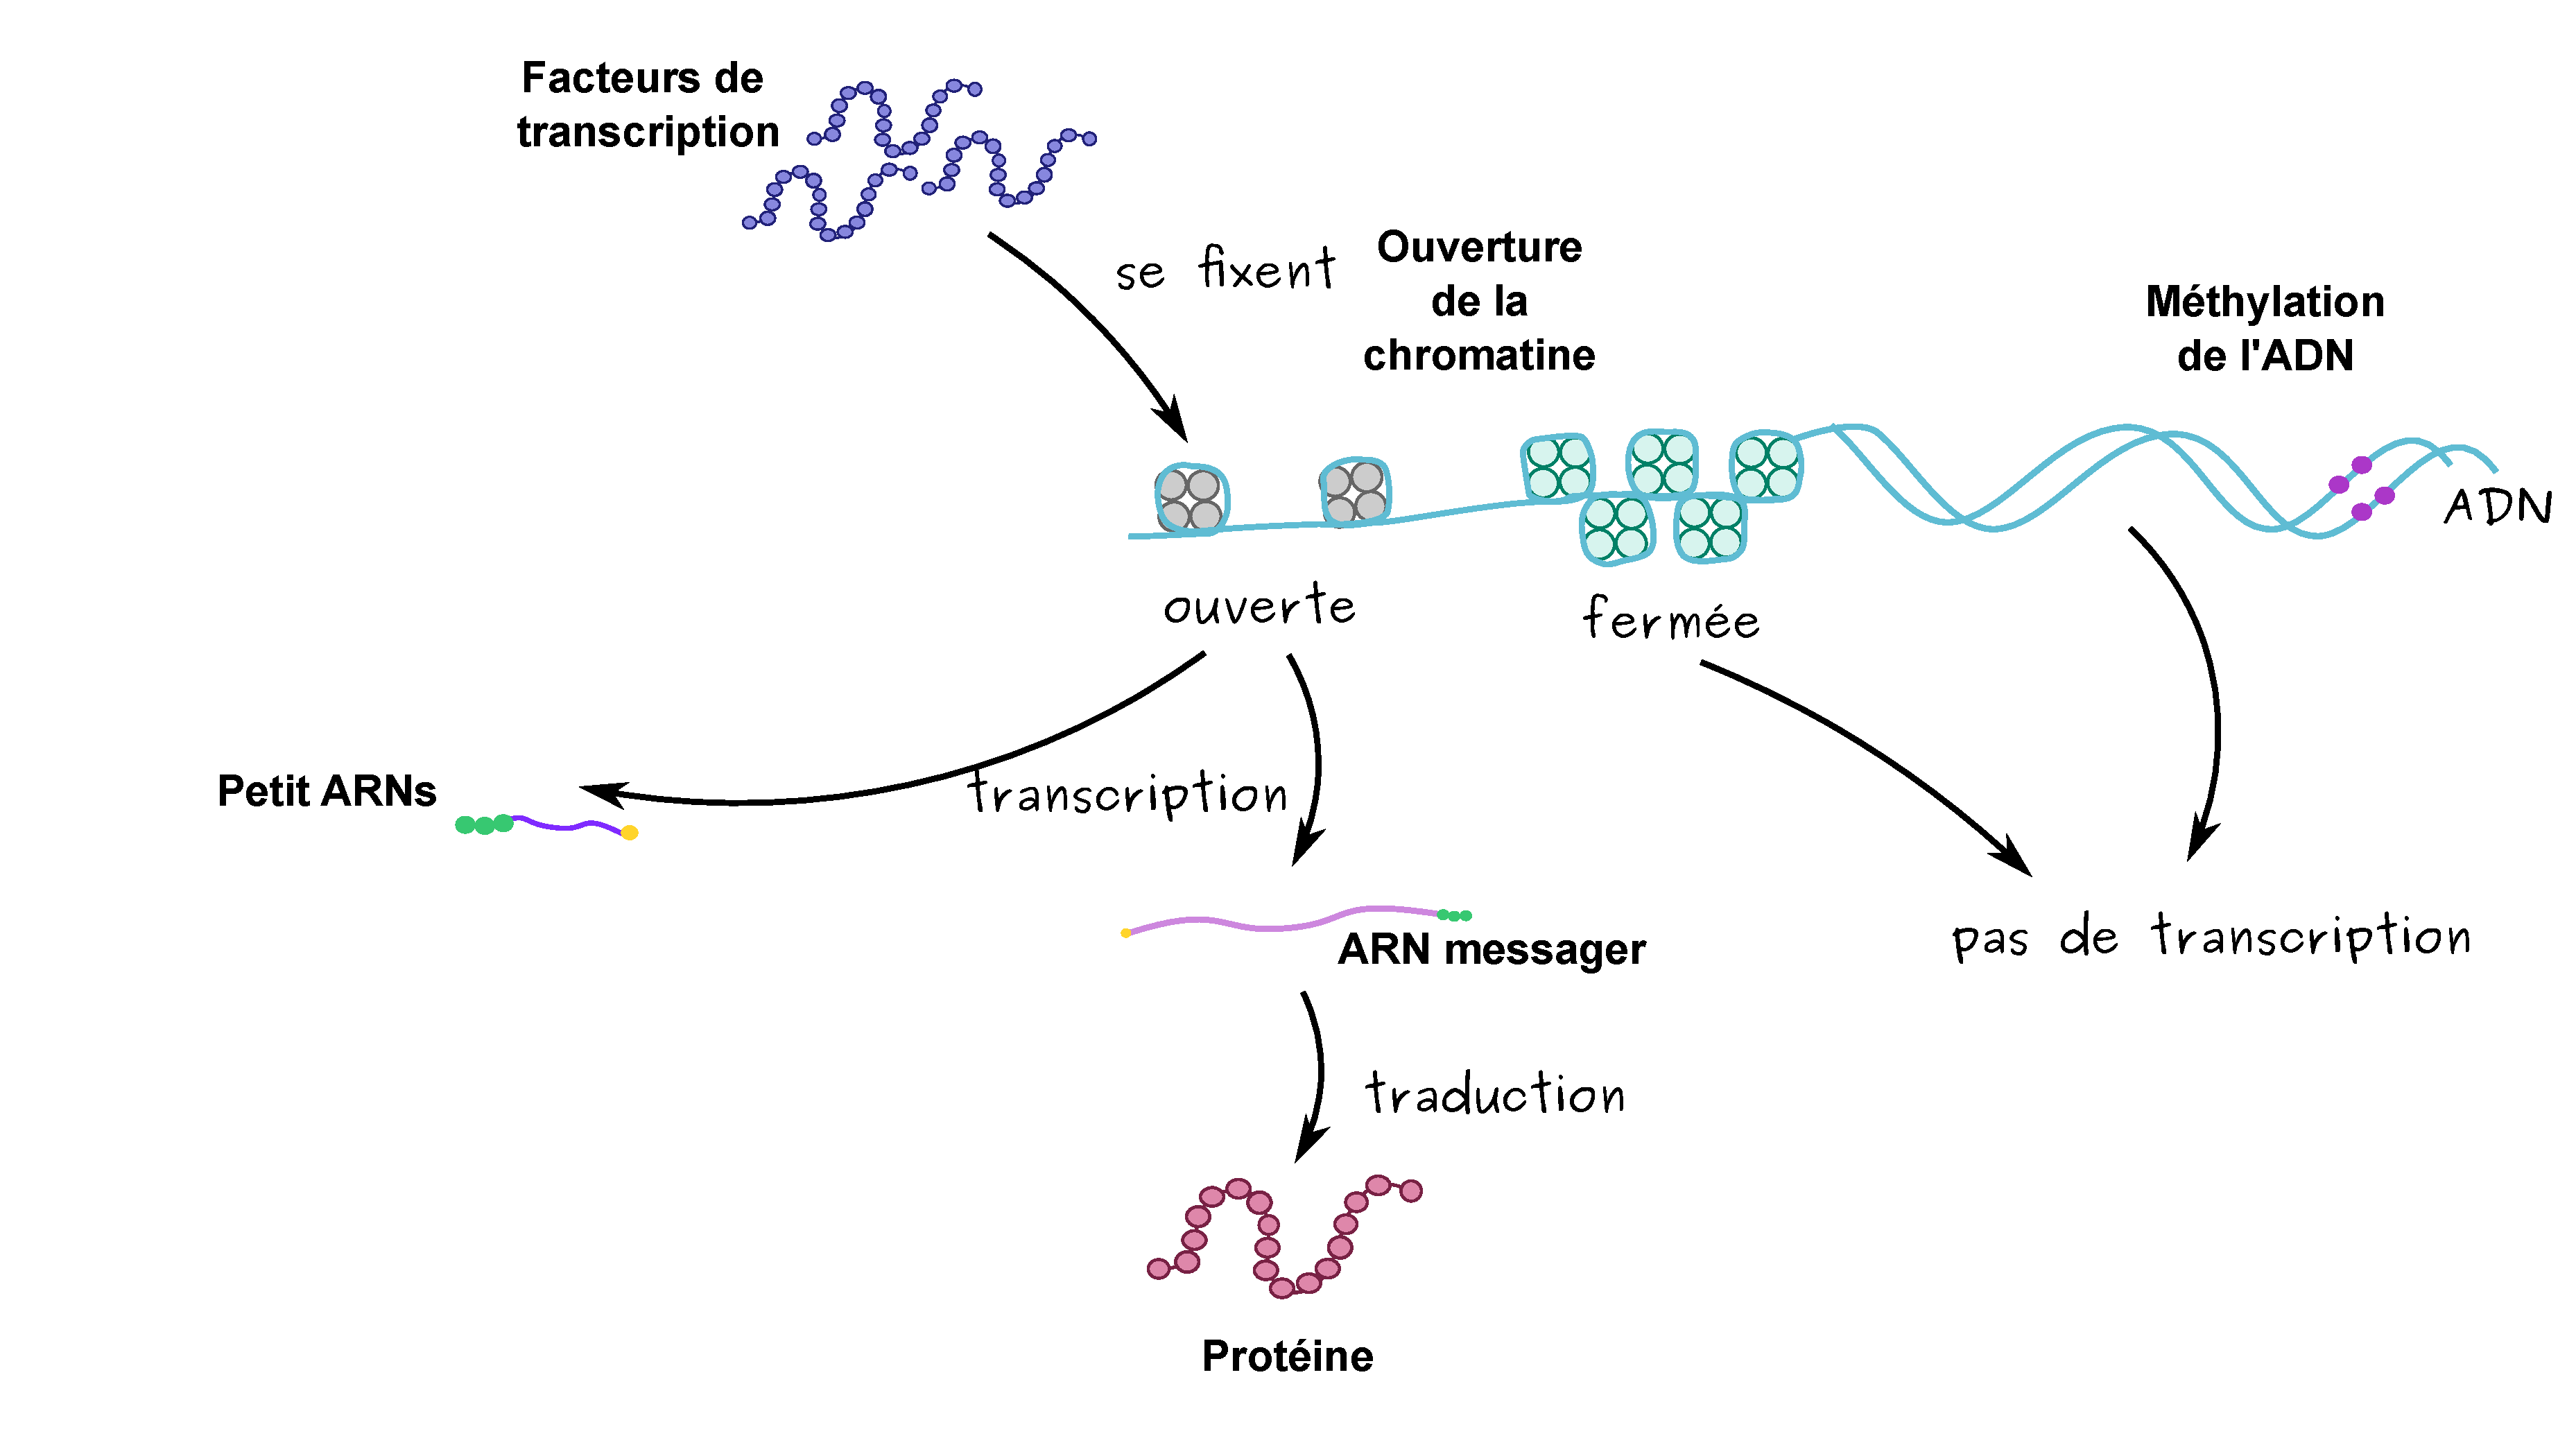
\includegraphics[width=0.9\linewidth]{schemas/gene_regulation_final_5.pdf}}%
\only<7>{%
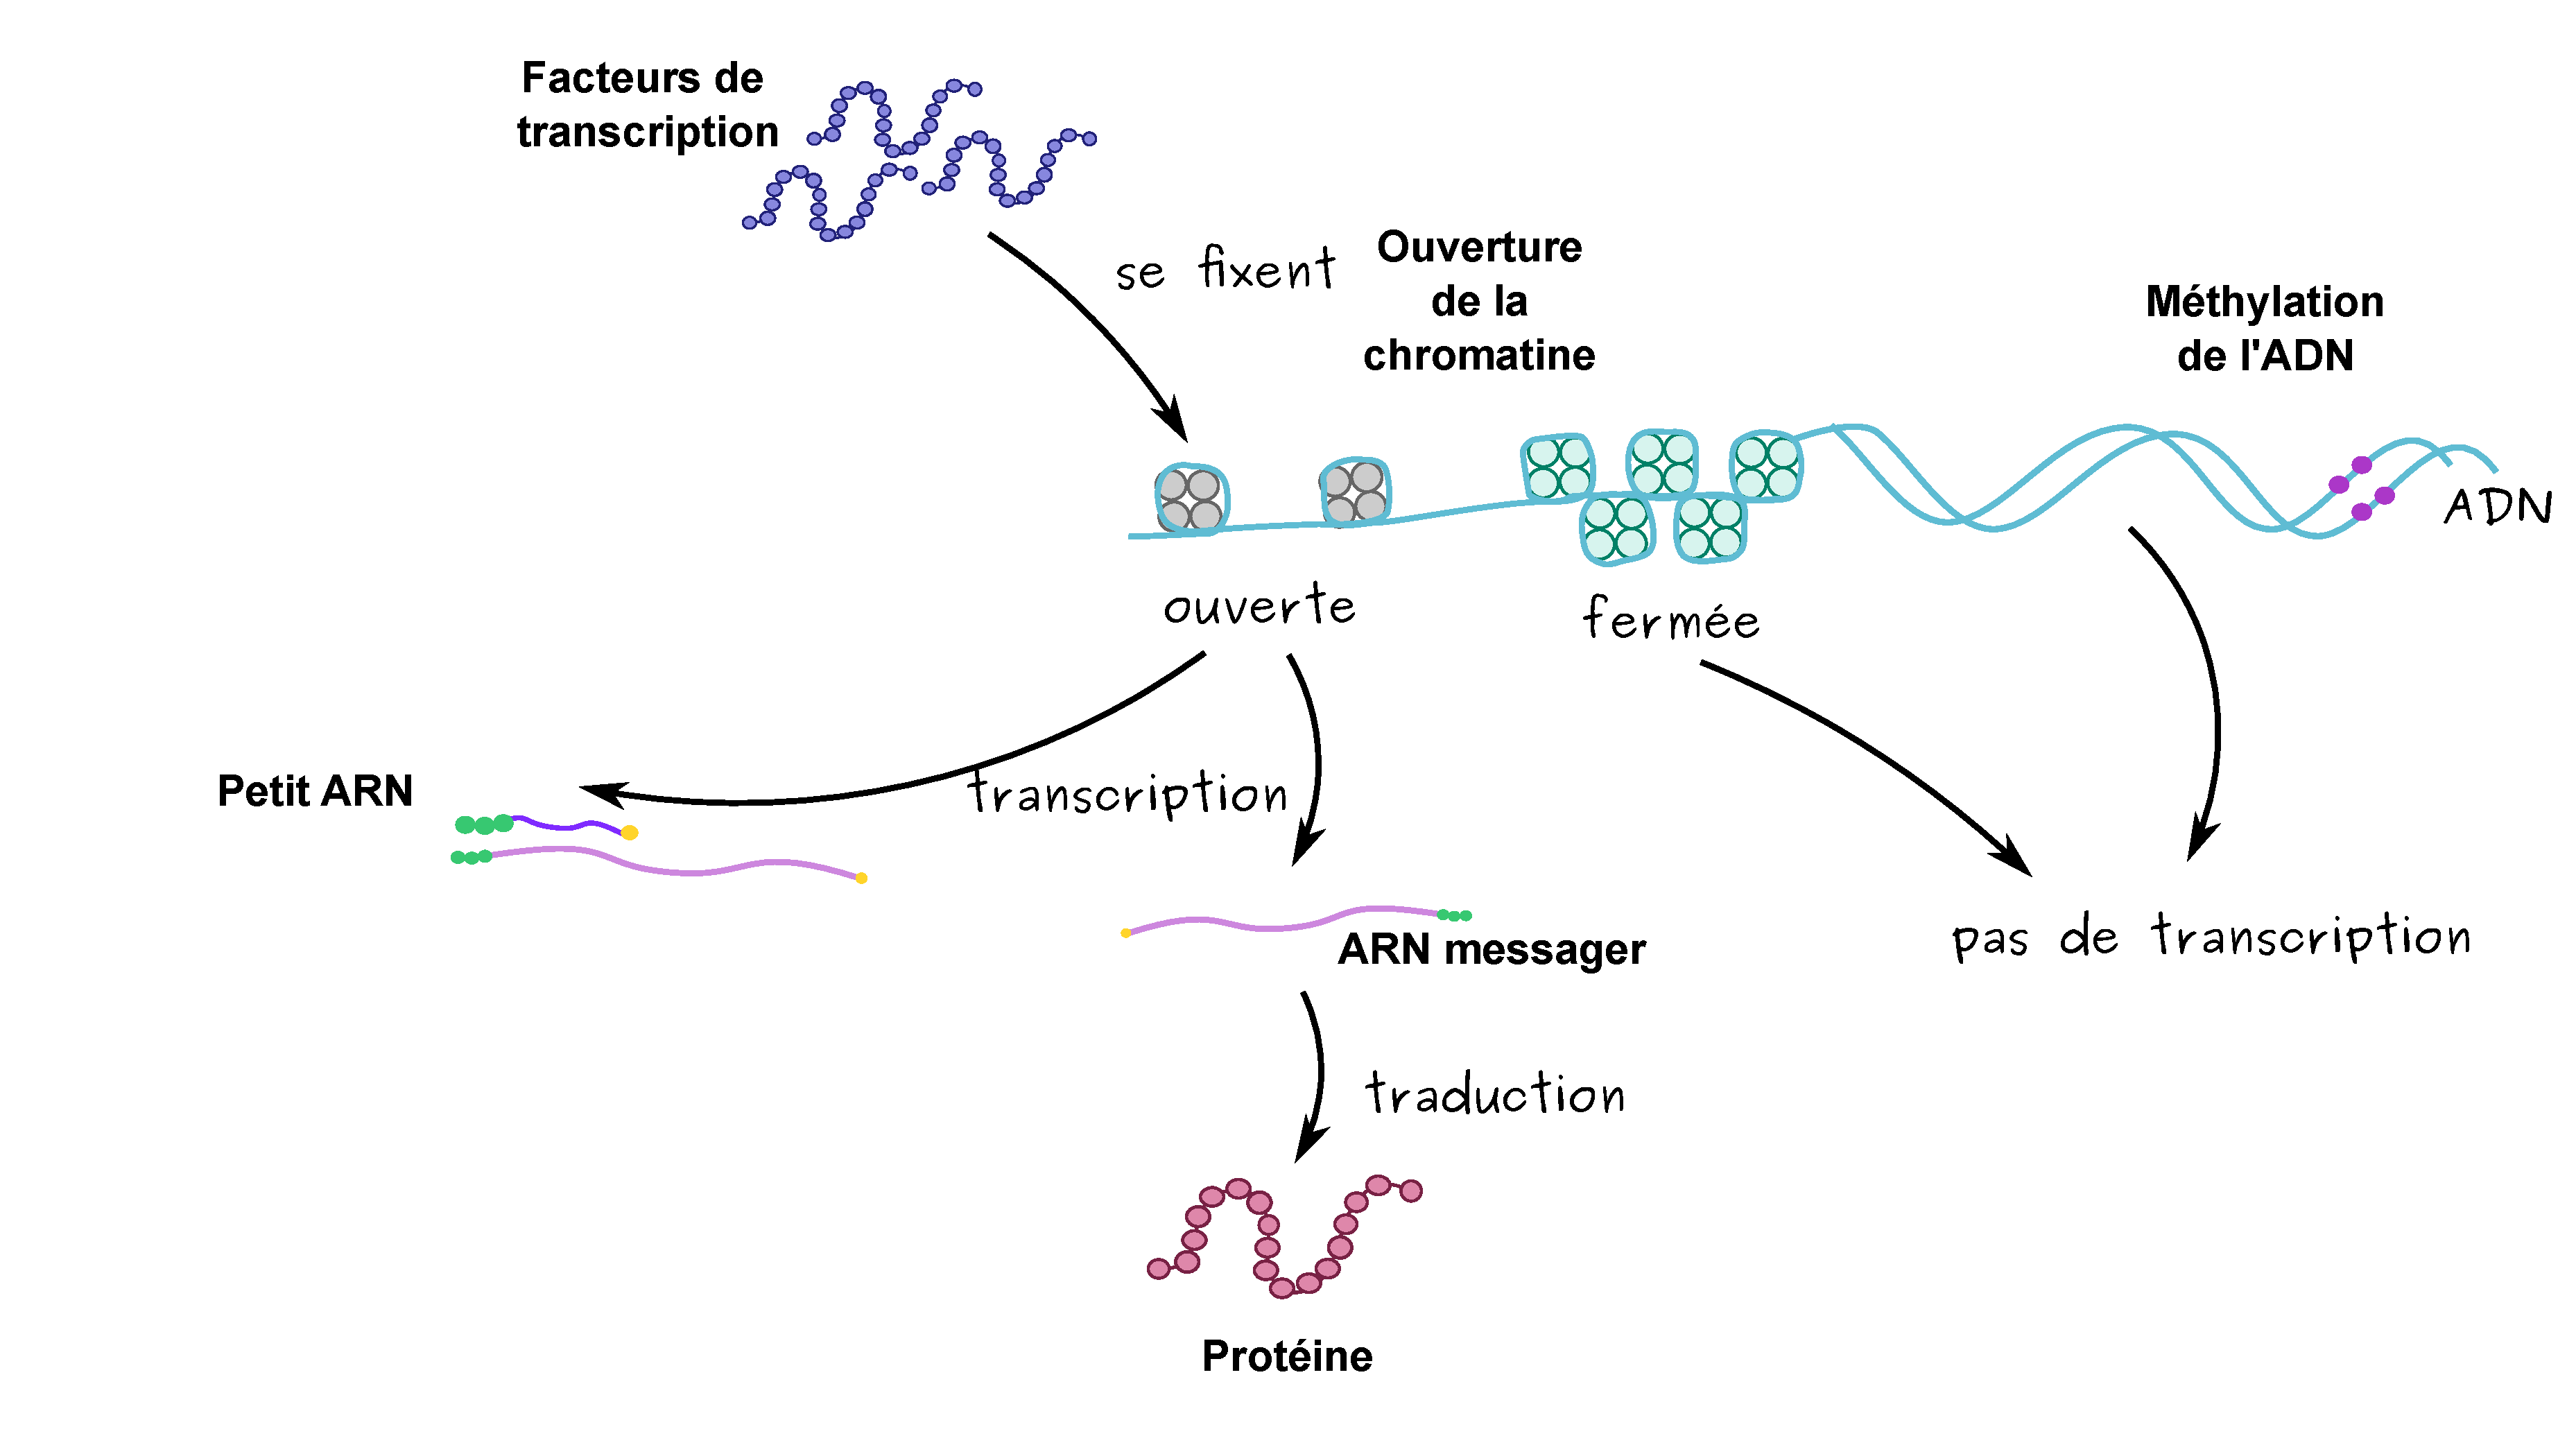
\includegraphics[width=0.9\linewidth]{schemas/gene_regulation_final_6.pdf}}%
\only<8>{%
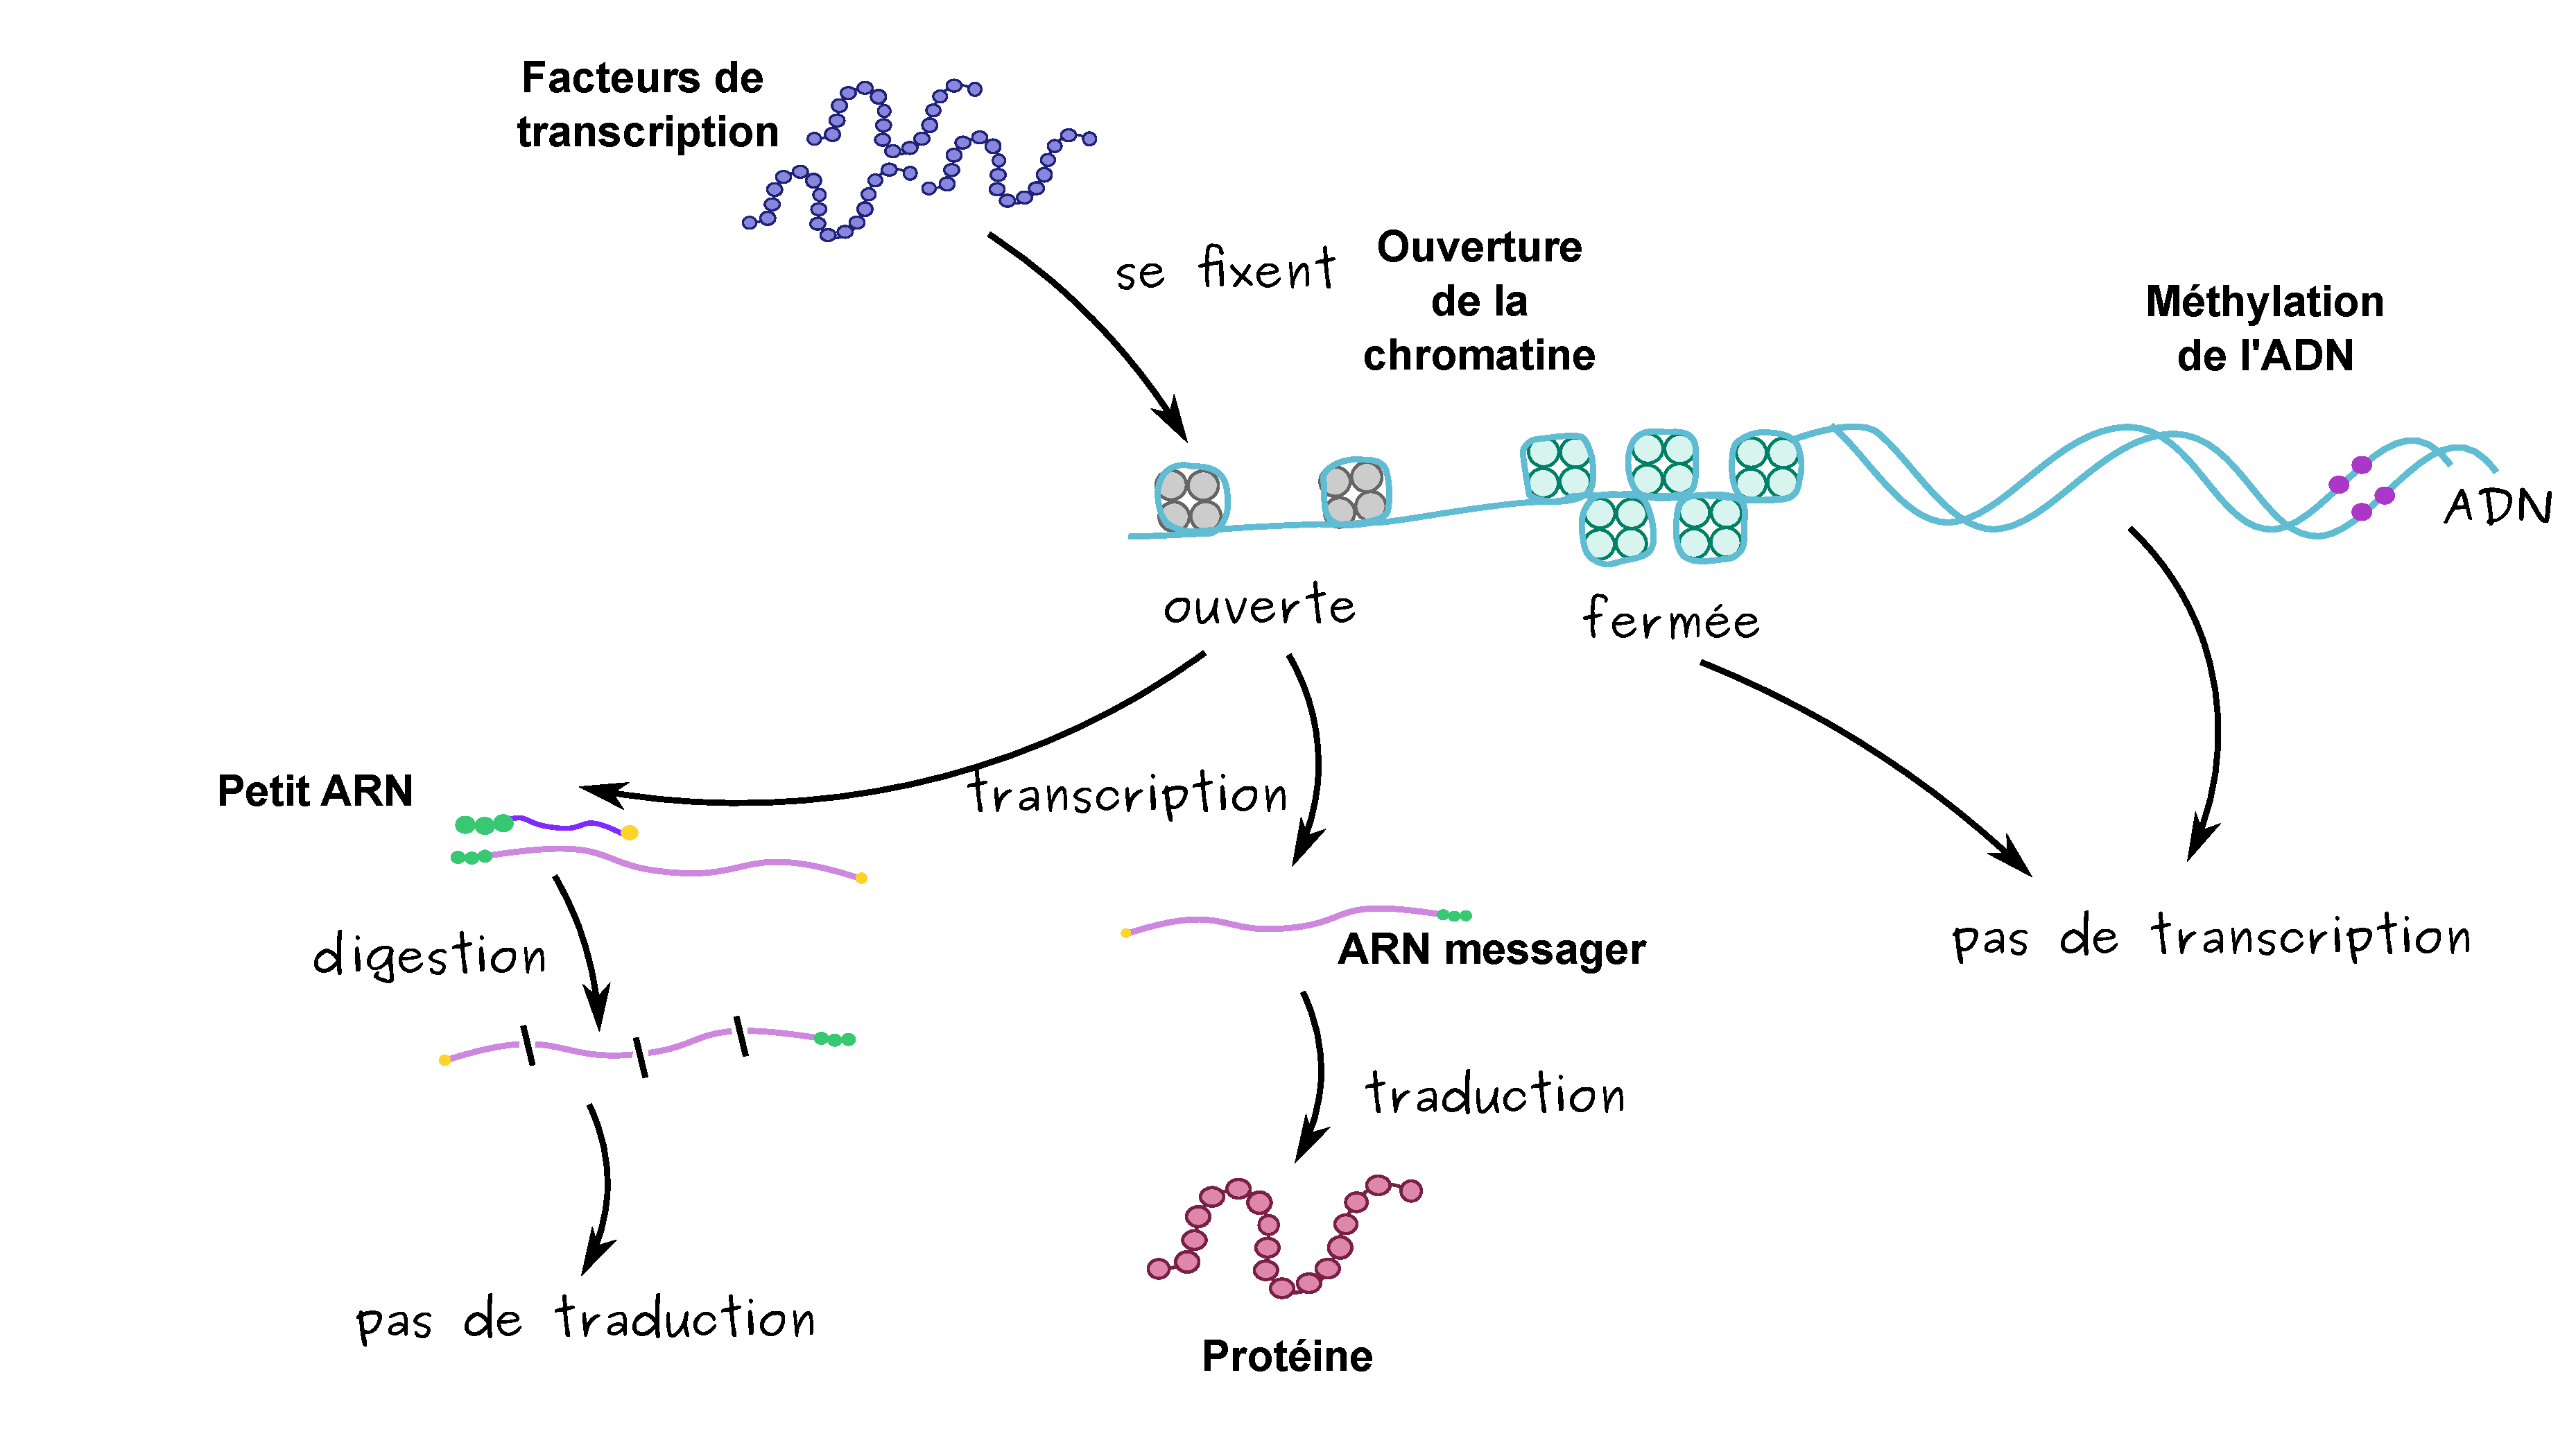
\includegraphics[width=0.9\linewidth]{schemas/gene_regulation_final_7.pdf}}%
\only<9>{%
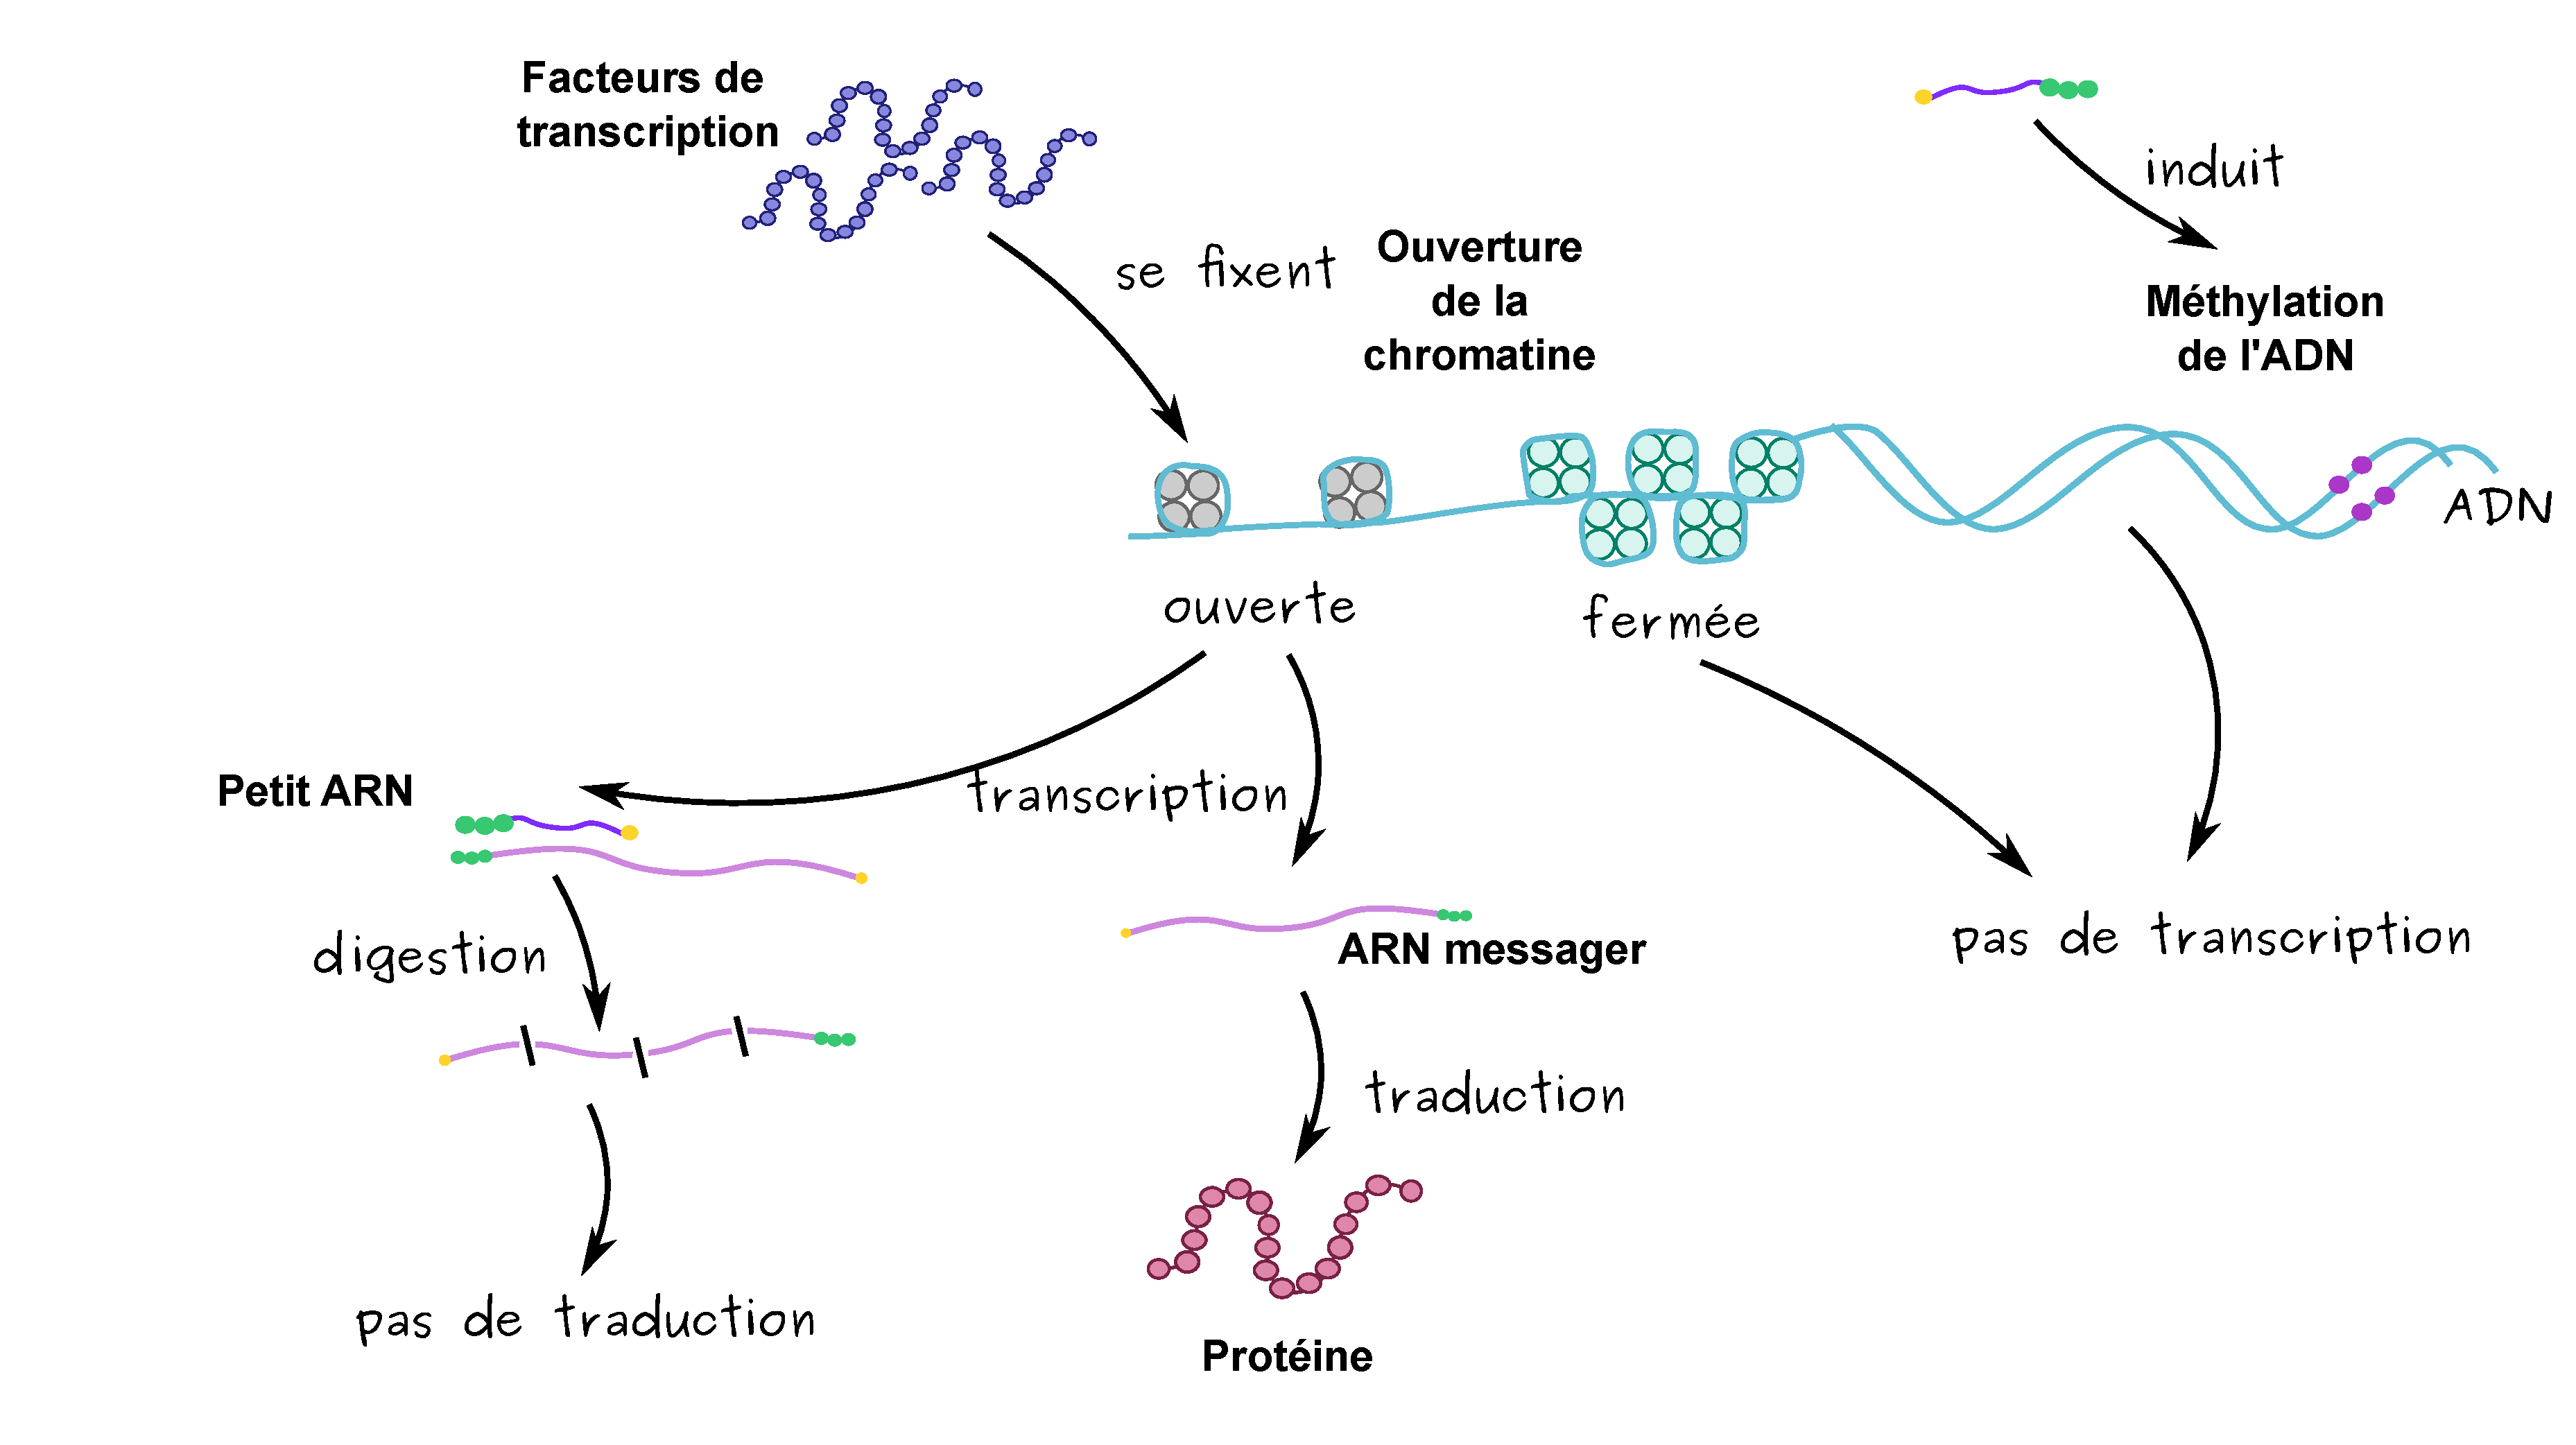
\includegraphics[width=0.9\linewidth]{schemas/gene_regulation_final_8.pdf}}%
\only<10>{%
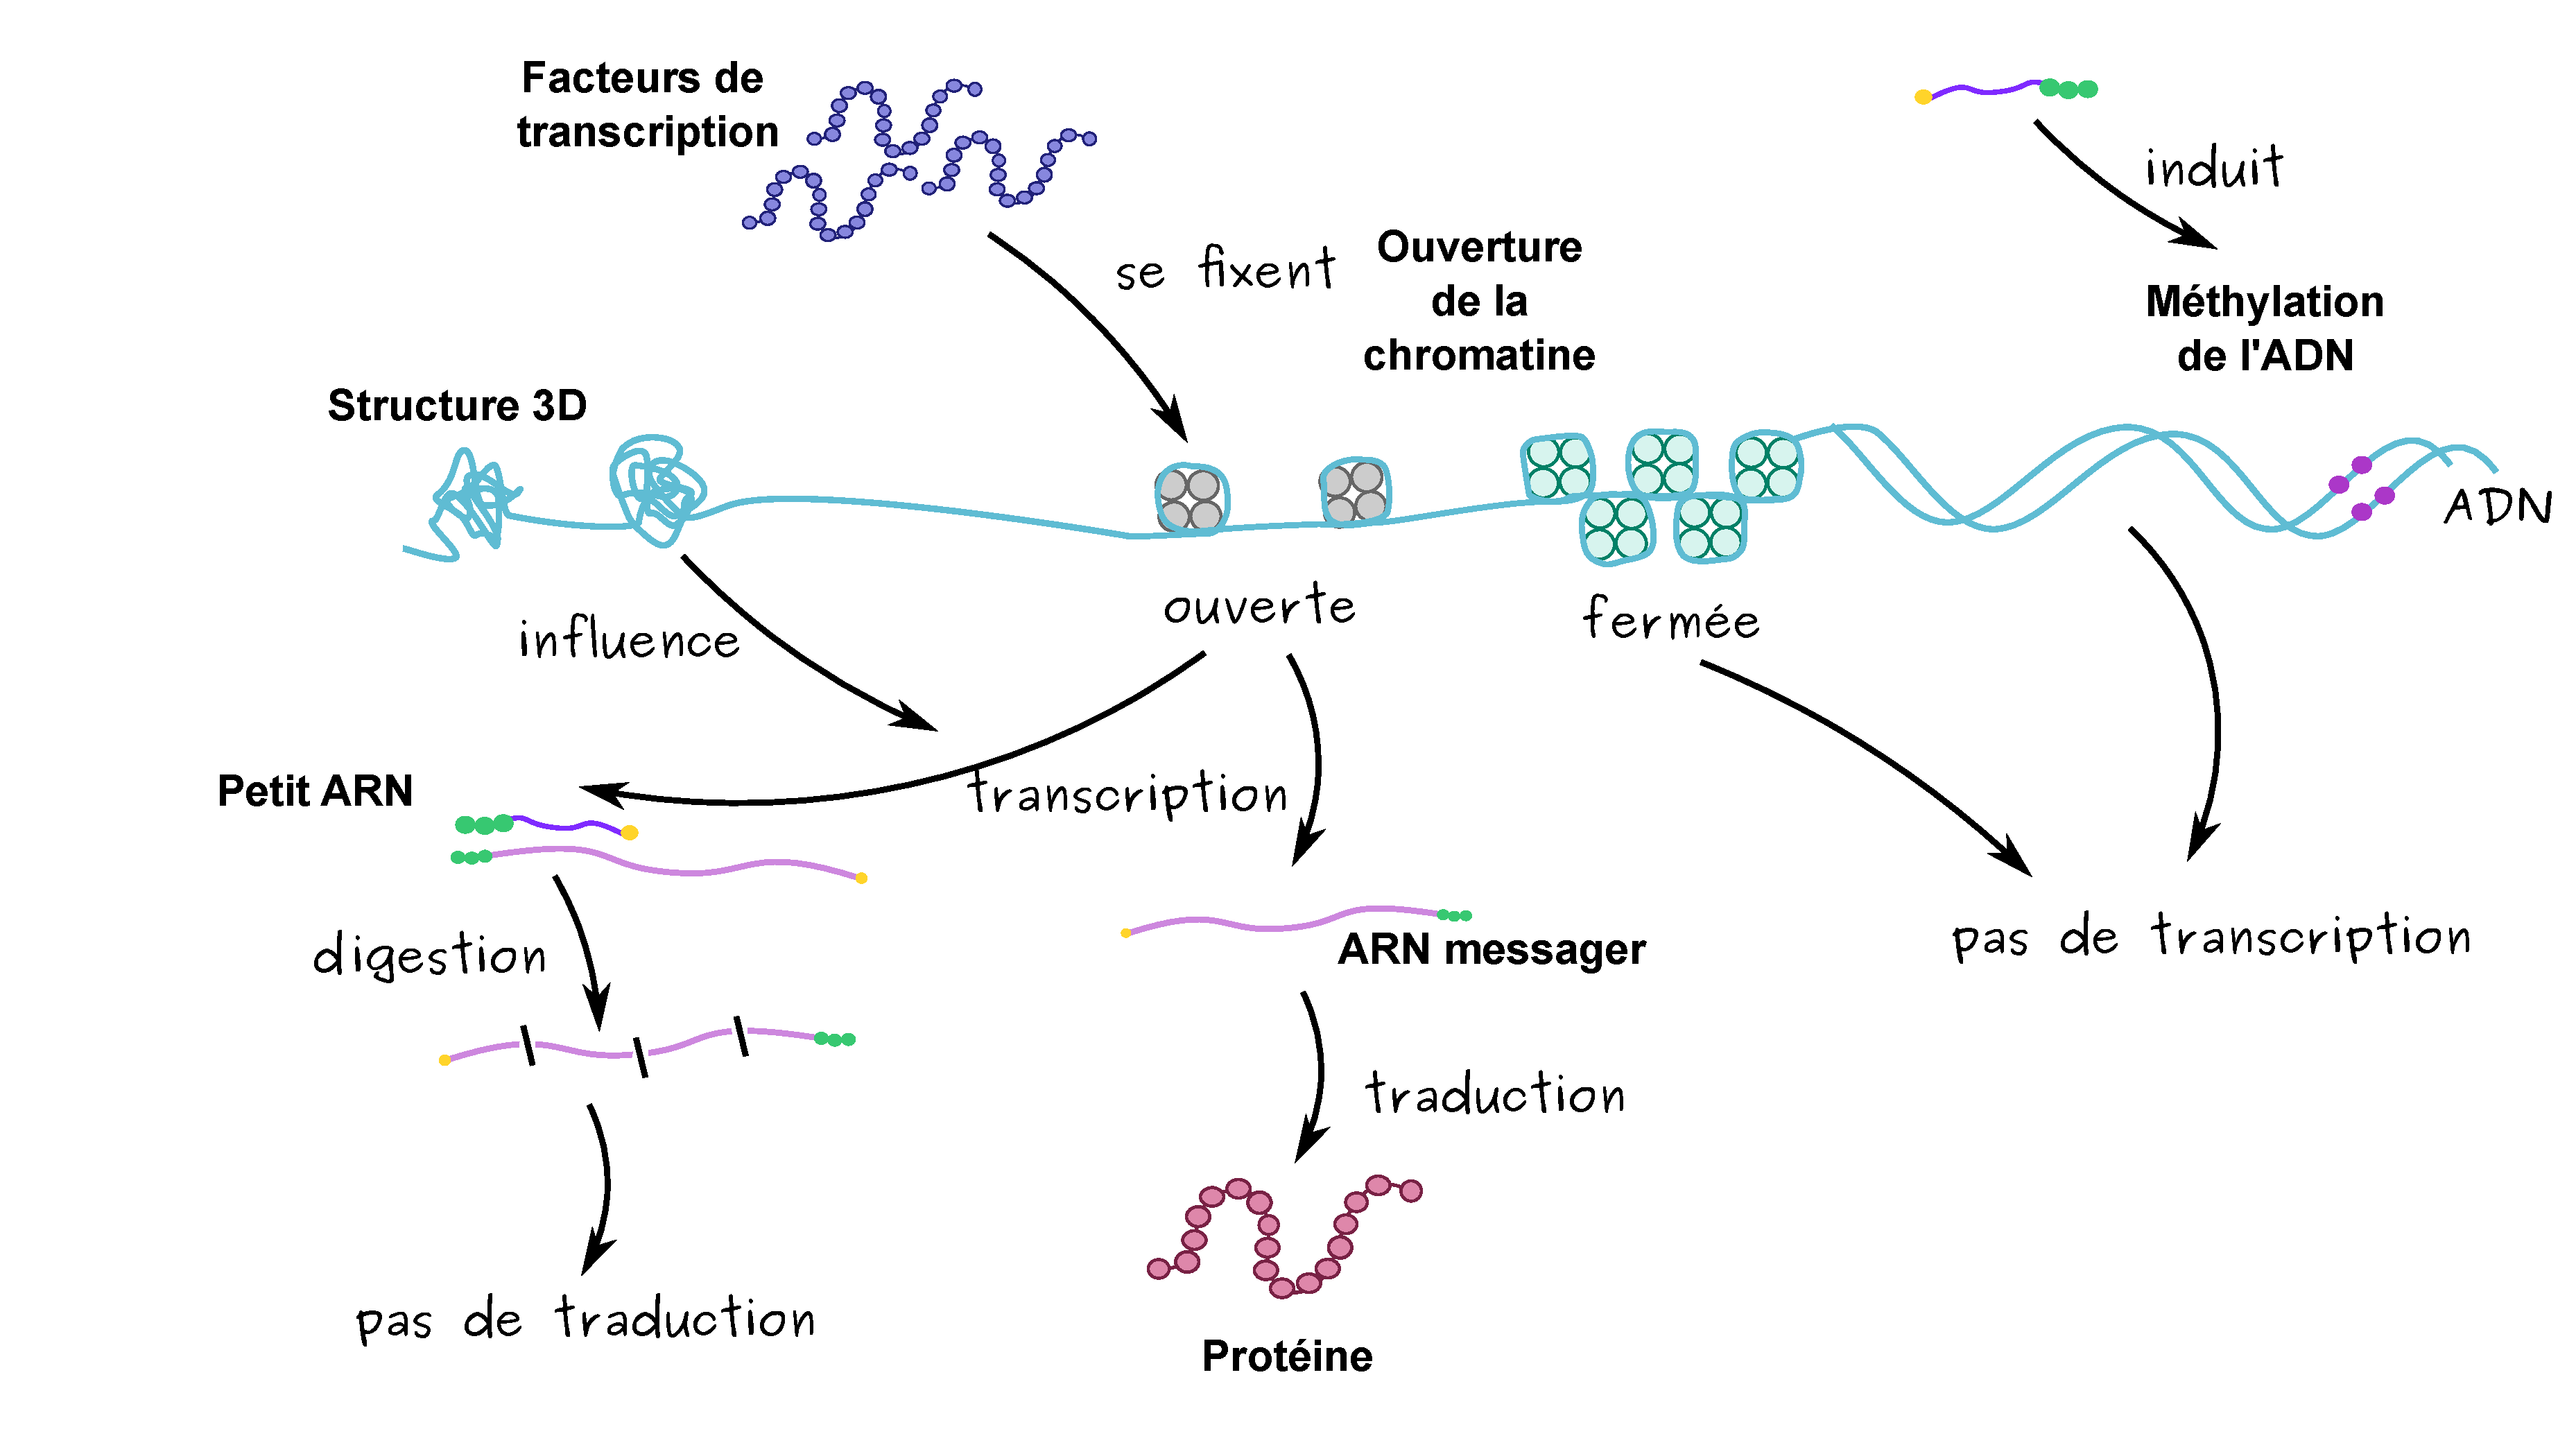
\includegraphics[width=0.9\linewidth]{schemas/gene_regulation_final_9.pdf}}%
\only<11->{%
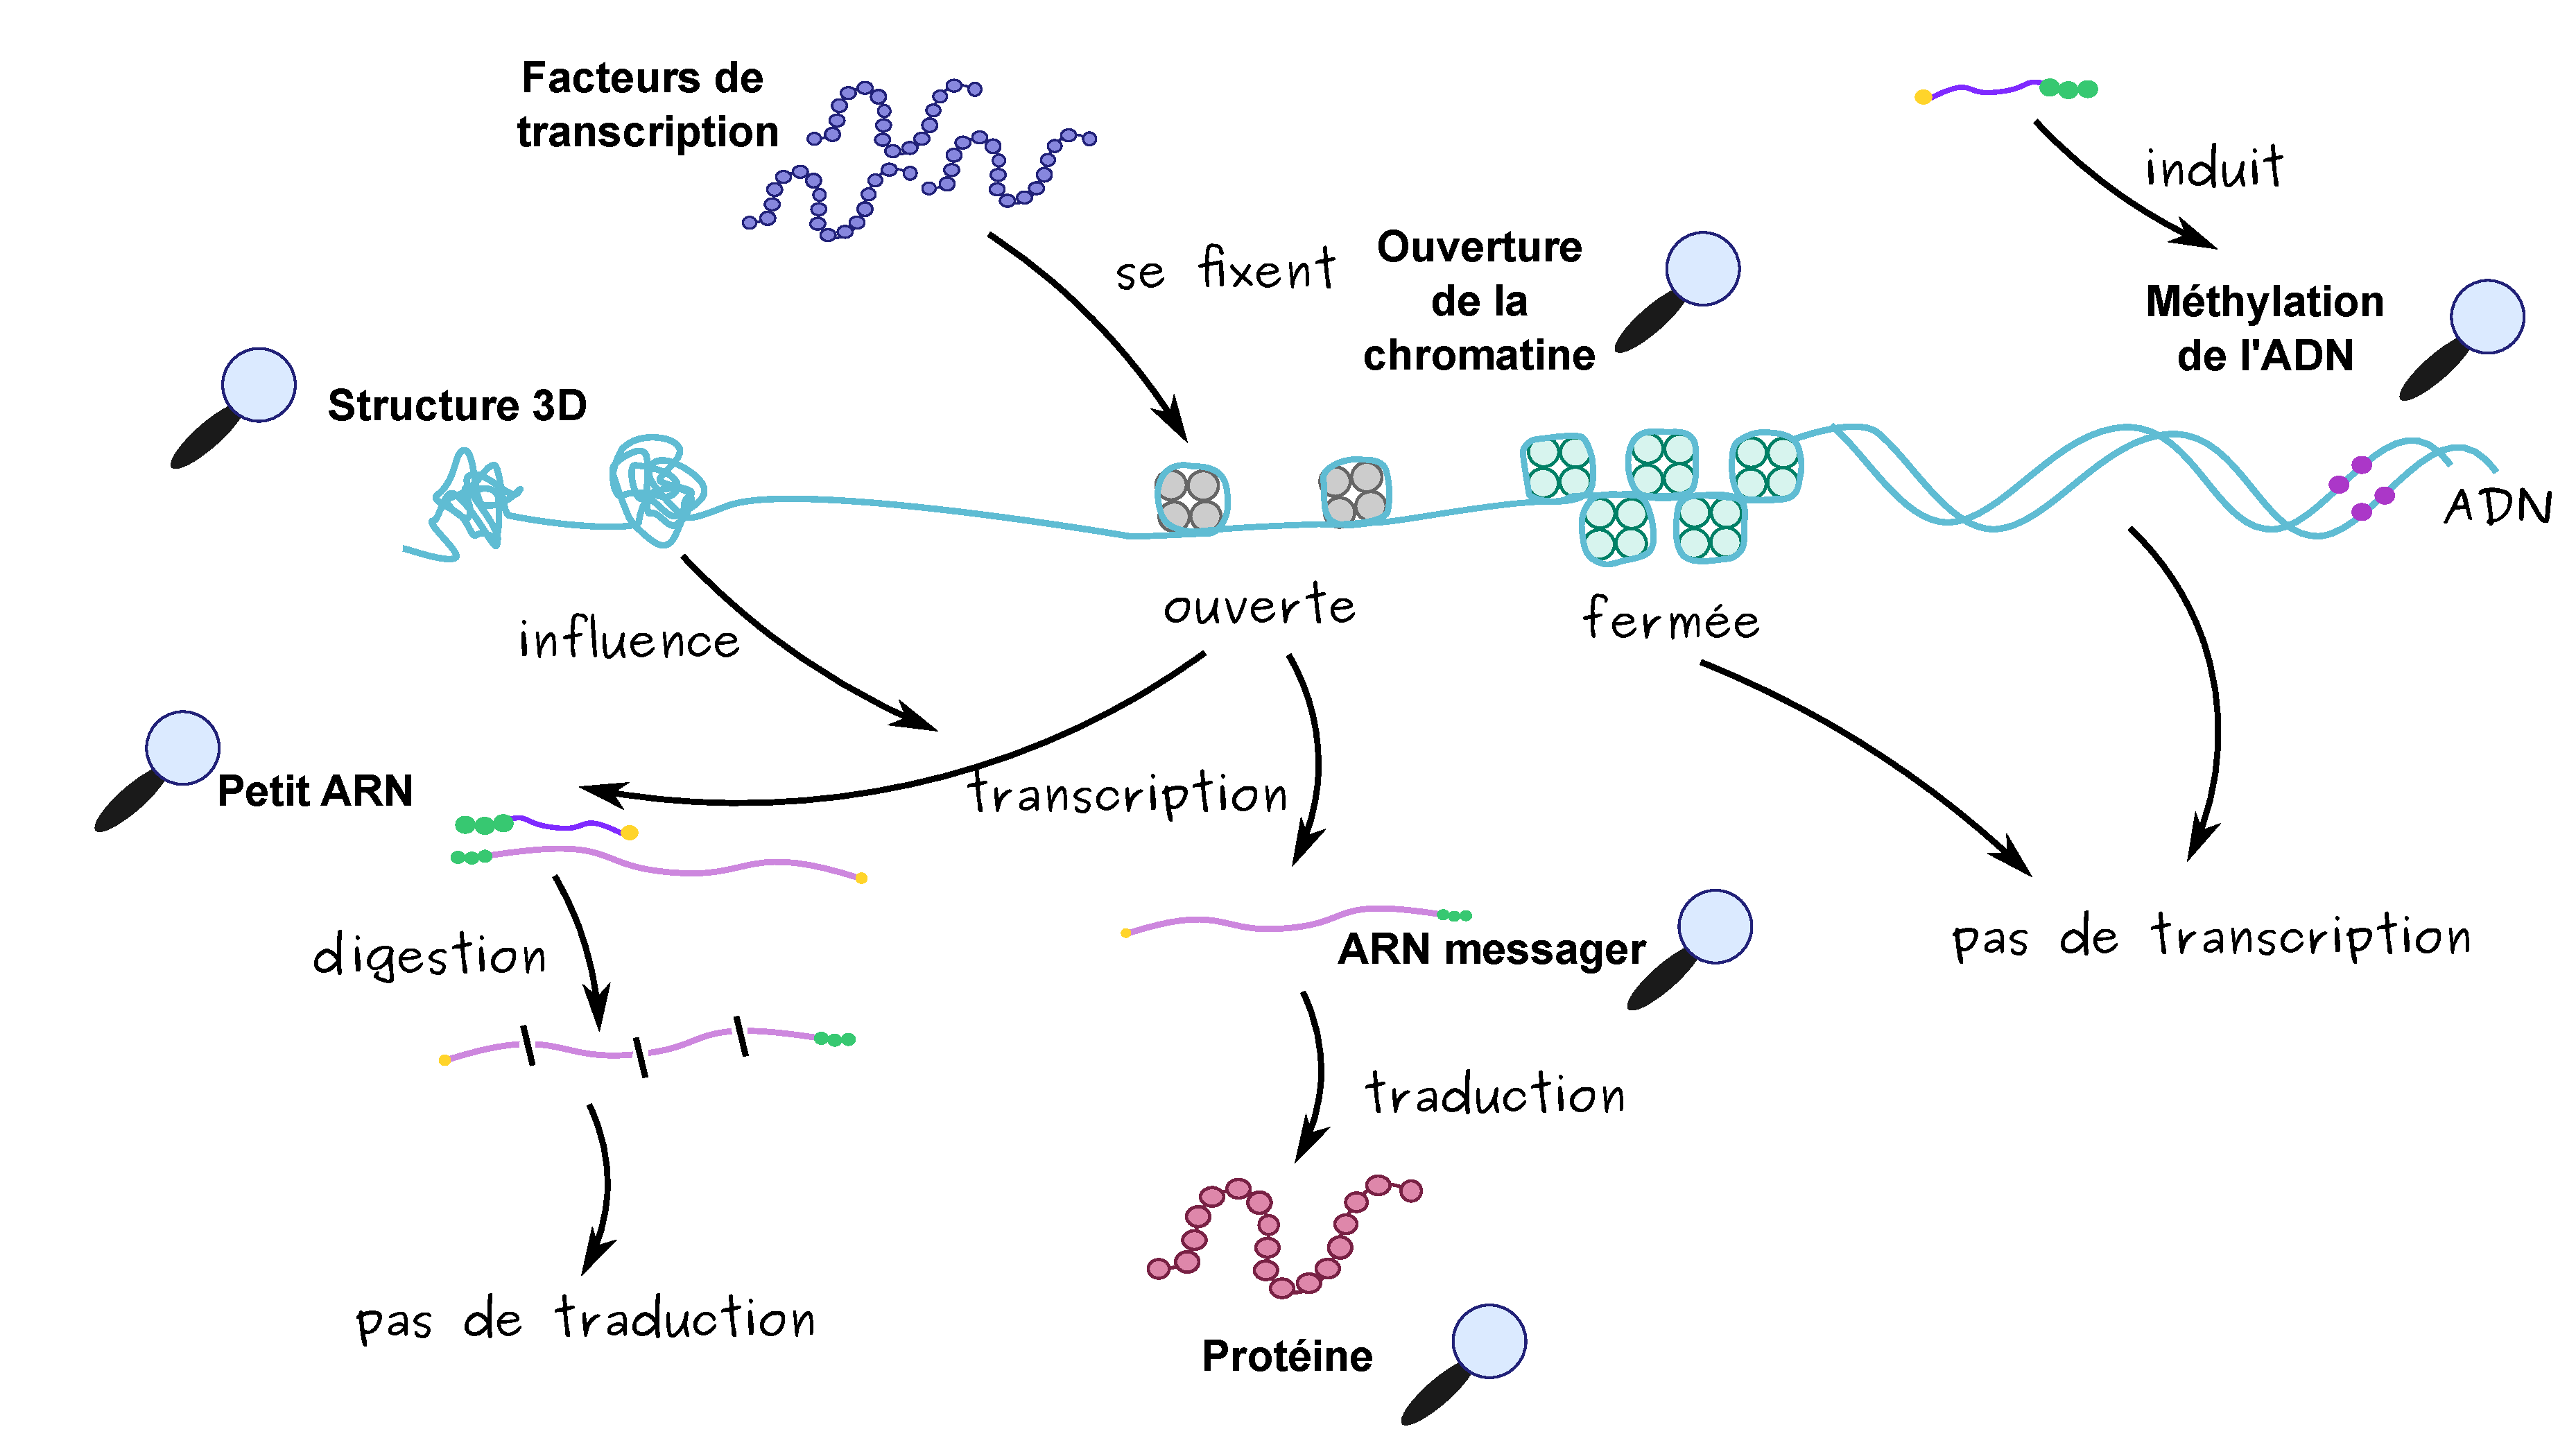
\includegraphics[width=0.9\linewidth]{schemas/gene_regulation_final_10.pdf}}
\end{figure}
\vspace{-0.4em}
\begin{overlayarea}{12cm}{5.5cm}%
\only<2-10>{%
\em
\centering
\vspace{1em}
\footnotesize
L'épigénétique est l'étude des mécanismes réversibles, transmissibles et
adaptifs impliqués dans la régulation des gènes.}
\only<11>{%
\vspace{-1.5em}
{\bf \footnotesize Les données épigénétiques : une vue multiple et globale sur la cellule}
\vskip-1.3ex
\rule{\dimexpr\paperwidth-1.5cm\relax}{0.4pt}
\begin{itemize}
\scriptsize
\item[-] Données hétérogènes. 
\item[-] Meilleure compréhension des mécanismes de régulation et
de dérégulation de l'expression génique.
\end{itemize}}
\only<12>{%
\vspace{-1.5em}
{\bf \footnotesize Le défi de l'épigénétique}
\vskip-1.3ex
\rule{\dimexpr\paperwidth-1.5cm\relax}{0.4pt}
\begin{itemize}
\scriptsize
\item[-] Peu d'échantillons, beaucoup de descripteurs souvent corrélés ($n <
p$).
\item[-] Données larges, difficiles à manipuler.
\item[-] Données hétéroscédastiques, bruitées, bruits de groupes.
\item[-] Modèle explicatif.
\end{itemize}
}
\end{overlayarea}

\end{frame}

\begin{frame}
\frametitle{Contributions principales}
\vspace{4em}
\hspace{2em}
\begin{tikzpicture}[overlay]

% Main horizontal line
\draw[ultra thick,->] (-1cm,0) -- (7.5,0);

% draw vertical lines
\foreach \x in {0,2,4,6}
    \draw[ultra thick] (\x cm,3pt) -- (\x cm,-3pt);
\foreach \x in {1,3,5,7}
    \draw (\x cm,2pt) --(\x cm,-2pt);

% draw names
\draw[ultra thick] (0,0) node[below=3pt,thick] {2012} node[above=3pt] {};
\draw[ultra thick] (2,0) node[below=3pt,thick] {2014} node[above=3pt] {};
\draw[ultra thick] (4,0) node[below=3pt, thick] {2016} node[above=3pt] {};
\draw[ultra thick] (6,0) node[below=3pt, thick] {2018} node[above=3pt] {};

% Hi-C
\draw [thick] (0.5 cm,2pt) -- (0.5cm,1.5cm);
\draw [fill=red](0.5,0) circle (0.1cm);
\draw [thick] (0.5cm,1.5cm) -- (1cm,1.75cm);
\draw [thick] (1cm,1.5cm) -- (1cm,2cm);
\draw [thick] (1cm, 1.75cm) node[right=3pt] {\parbox[t]{3.5cm}{\scriptsize {\bf
{\em Structure 3D du génome}}
\begin{itemize}[leftmargin=*]
\tiny
\item[-]{
\only<1-4>{%
\bf {\color{red} Varoquaux} et al., \scalebox{.7}{Bioinformatics (2014)}}
\only<5->{%
\bf \color{blue} Varoquaux et al., \scalebox{.7}{Bioinformatics (2014)}}
}
\item[-]{%
\only<1-4>{\bf Servant, {\color{red} Varoquaux} et al.
\scalebox{.7}{Genome Biology (2015)}}
\only<5->{\bf \color{blue} Servant, Varoquaux et al. \scalebox{.7}{Genome Biology (2015)}}
}
\item[-]{%
\only<1-4>{%
\bf {\color{red} Varoquaux} et al. \scalebox{.7}{NAR (2015)}}
\only<5->{%
\bf \color{blue} Varoquaux et al. \scalebox{.7}{NAR (2015)}}}
\item[-]{%
\only<1-4>{%
\bf Servant$^*$, {\color{red} Varoquaux$^*$} et al. \scalebox{.7}{BMC bioinformatics
(2018)}}
\only<5->{%
\bf \color{blue} Servant$^*$, Varoquaux$^*$ et al. \scalebox{.7}{BMC bioinformatics
(2018)}}
}
\item[-]{%
\only<1-4>{\bf \color{gray} {\color{red} Varoquaux}, Servant
\scalebox{.7}{JOSS (accepté)}}
\only<5->{\bf \color{blue} Varoquaux, Servant \scalebox{.7}{JOSS (accepté)}}}
\item[-]{%
\only<1-4>{%
\bf \color{gray}  {\color{red} Varoquaux} et al. \scalebox{.7}{(en
préparation)}}
\only<5->{%
\bf \color{blue} Varoquaux et al. \scalebox{.7}{(en préparation)}}
}
\end{itemize}
}
};

% P. falciparum
\only<2->{
\draw [thick] (1 cm,2pt) -- (1cm,-3.25cm);
\draw [fill=red](1,0) circle (0.1cm);
\draw [thick] (1cm,-3.25cm) -- (1.5cm,-3.5cm);
\draw [thick] (1.5cm,-3.25cm) -- (1.5cm,-3.75cm);
\draw [thick] (1.5cm, -3.5cm) node[right=3pt] {\parbox[t]{5cm}{\scriptsize {\bf
\em Application santé :  P. falciparum}
\begin{itemize}[leftmargin=*]
\tiny
\item[-]{%
\only<1-4>{%
\bf Ay$^*$, Bunnik$^*$, {\color{red} Varoquaux$^*$} et al.,
\scalebox{.7}{Genome Research (2014)}}
\only<5->{%
\bf \color{green}Ay$^*$, Bunnik$^*$, Varoquaux$^*$ et al., \scalebox{.7}{Genome Research(2014)}}}
\item[-]{%
\only<1-4>{\bf Ay$^*$, Bunnik$^*$, {\color{red} Varoquaux} et al.
\scalebox{.7}{Bioessays (2014)}}
\only<5->{\bf \color{green} Ay$^*$, Bunnik$^*$, Varoquaux et al.
\scalebox{.7}{Bioessays (2014)}}}
\item[-]{%
\only<1-4>{\bf {\color{red} Varoquaux} \scalebox{.7}{International journal of
Biostatistics (2018)}}}
\only<5->{\bf \color{blue} Varoquaux \scalebox{.7}{International journal of
Biostatistics (2018)}}
\item[-] {%
\only<1-4>{\bf Bunnik$^*$, Cook$^*$, {\color{red} Varoquaux} et al.
\scalebox{.7}{Nature Communication (2018)}}
\only<5>{\bf \color{green}Bunnik$^*$, Cook$^*$, Varoquaux et al.
\scalebox{.7}{Nature Communication (2018)}}}
\end{itemize}
}
};
}
% EPICON
\only<3->{
\draw [thick] (4.5 cm,2pt) -- (4.5cm,-1.75cm);
\draw [fill=red](4.5,0) circle (0.1cm);
\draw [thick] (4.5cm,-1.75cm) -- (4.75cm,-2cm);
\draw [thick] (4.75cm, -1.75cm) -- (4.75cm,-2.25cm);
\draw [thick] (4.75cm, -1.75cm) node[right=3pt] {\parbox[t]{6cm}{\scriptsize {\bf
\em Analyse fonctionnelle \& expression génique}
\begin{itemize}[leftmargin=*]
\tiny
\item[-]{%
\only<1-4>{\bf Giordano$^*$, Liu$^*$, {\color{red} Varoquaux$^*$}, et
al. \scalebox{.7}{NIPS AABIW (2017)}}
\only<5->{\bf \color{blue} Giordano$^*$, Liu$^*$, Varoquaux$^*$, et
al. \scalebox{.7}{NIPS AABIW (2017)}}
}
\item[-]{%
\only<1-4>{%
\bf \color{gray} {\color{red} Varoquaux$^*$}, Cole$^*$, Gao$^*$ et al.
\scalebox{.7}{(soumis)}}
\only<5->{%
\bf \color{green} Varoquaux$^*$, Cole$^*$, Gao$^*$ et al
\scalebox{.7}{(soumis)}
}}
\item[-]{%
\only<1-4>{%
\bf \color{gray} {\color{red} Varoquaux}, Purdom \scalebox{.7}{(en
préparation)}}
\only<5->{%
\bf \color{blue} Varoquaux, Purdom \scalebox{.7}{(en préparation)}}}
\item[-] {%
\only<1-4>{%
\bf \color{gray} {\color{red} Varoquaux$^*$}, DeGraaf$^*$ et al.
\scalebox{.7}{(en préparation)}}
\only<5->{%
\bf \color{blue} Varoquaux$^*$, DeGraaf$^*$ et al. \scalebox{.7}{(en
préparation)}}}
\end{itemize}}
};}

% EMBeR
\only<4->{
\draw [thick] (5.5 cm,2pt) -- (5.5cm,0.5cm);
\draw [fill=red](5.5,0) circle (0.1cm);
\draw [thick] (5.5cm,.5cm) -- (5.75cm,0.75cm);
\draw [thick] (5.75cm, .5cm) -- (5.75cm,1cm);
\draw [thick] (5.75cm, 1cm) node[right=3pt] {\parbox[t]{5cm}{\scriptsize {\bf
\em Communauté des logiciels libres}
\begin{itemize}[leftmargin=*]
\tiny
\item[-]{%
\only<1-4>{\bf Geiger, {\color{red} Varoquaux} et al. \scalebox{.7}{(CSCW
2018)}}
\only<5->{\bf Geiger, Varoquaux et al. \scalebox{.7}{CSCW (2018)}}}
\item[-]{%
\only<1-4>{\bf \color{gray}  Paxton, {\color{red} Varoquaux} et al.
\scalebox{.7}{(en préparation)}}
\only<5->{\bf Paxton, Varoquaux et al. \scalebox{.7}{(en préparation)}}}
\end{itemize}
}
};}
%
\only<5->{%
\draw [thick] (7.5cm, -4.1cm) node[right=1pt] {%
\parbox[t]{5cm}{%
\fontsize{2.5}{4}
\tiny
\bf
{\color{blue} Développement méthodologique} \\
{\color{green} Collaboration en biologie} \\
{\color{black} Collaboration en sciences humaines} \\
}};}

\end{tikzpicture}
\begin{overlayarea}{12cm}{2cm}
\vspace{-4cm}
\begin{flushright}
\only<4->{%

\includegraphics[width=0.15\linewidth]{images/matplotlib.png} \quad

\includegraphics[width=0.12\linewidth]{images/scikit-learn.png} \quad

\includegraphics[width=0.15\linewidth]{images/scikit-image.png} \quad
}
\end{flushright}
\end{overlayarea}

\end{frame}



\begin{frame}
\frametitle{Contribution I\quad Inférence de la structure 3D du génome}

\begin{figure}
\centering
\includegraphics[width=0.5\linewidth]{images/counts_pfalc.pdf}
\end{figure}
\begin{flushright}
\tiny Ay$^*$, Bunnik$^*$, {\color{red} Varoquaux$^*$} et
al, Genome Research (2014)
\end{flushright}


\begin{overlayarea}{12cm}{4cm}
\only<2->{%
{\bf \small Les données Hi-C}
\footnotesize
\vskip-1.3ex
\rule{\dimexpr\paperwidth-1.5cm\relax}{0.4pt}
\begin{itemize}
\item[-] Matrices de très grande dimension à haute résolution (humain $3e10^6 \times
3e10^6$)
\item[-] Mesure bruitée et indirecte de la structure 3D du génome
\end{itemize}
}
\end{overlayarea}
\end{frame}

\begin{frame}
\frametitle{Contribution I\quad Inférence de la structure 3D du génome}

\begin{overlayarea}{12cm}{4cm}
\only<1->{%
\begin{center}
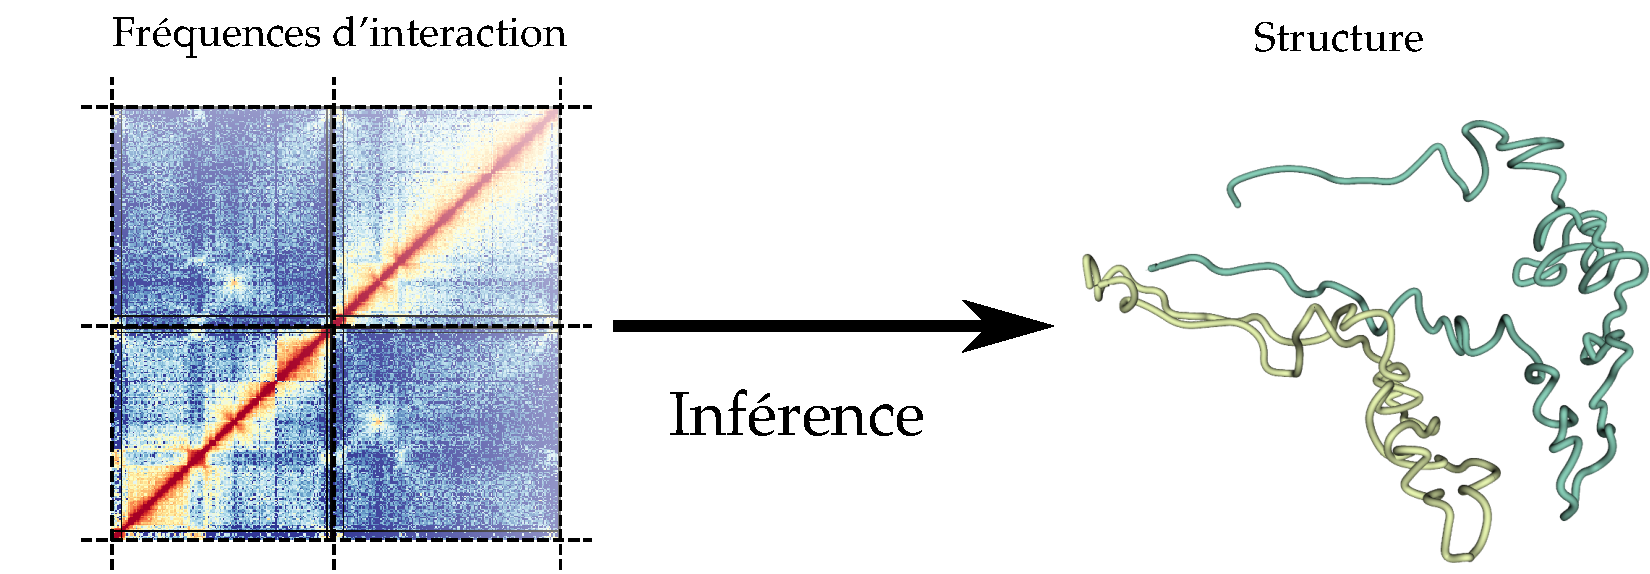
\includegraphics[width=0.9\linewidth]{figures/exemple_structure_inference.pdf}
\end{center}
}
\end{overlayarea}

\begin{overlayarea}{12cm}{4cm}
\only<2->{%
{\bf \small Une approche statistique pour inférer une structure
tridimensionnelle}
\vskip-1.3ex
\rule{\dimexpr\paperwidth-1.5cm\relax}{0.4pt}
}
\only<2->{%
\begin{itemize}
\only<2>{%
\small
\item[-] Modélisation de la fréquence d'interaction  entre les
éléments $i$ et $j$ :
{\large
\begin{equation*}
\underbrace{c_{ij}}_{\text{\tiny fréquence d'interaction}} \sim
\quad
\text{NB}\Big(\underbrace{\beta_{ij}}_{\text{\tiny bias}}
\underbrace{\|x_i - x_j\|_2^\alpha}_{\text{\tiny distance}},
\underbrace{r(\|x_i - x_j\|_2, \beta_{ij}, \alpha)}_{\text{\tiny
dispersion}}\Big)
\end{equation*}}}
\only<3->{%
\small
\item[-] Maximisation de la vraisemblance ($d_{ij} = \|x_i - x_j\|_2$)
  \begin{equation*}
  \hspace{-2.5em}
  \underset{x_1, \dots x_n}{\text{max}}\quad\log\Big(\frac{\Gamma(c_{ij} +
  \beta_{ij} r(d_{ij}^\alpha))}{\Gamma(c_{ij} +
  1)\Gamma(\beta_{ij} r(d_{ij}^\alpha))} \Big(\frac{d_{ij}^\alpha}{r(d_{ij}^\alpha) + d_{ij}^\alpha}\Big)^{c_{ij}}
  \Big(\frac{r(d_{ij}^\alpha
  )}{r(d_{ij}^\alpha) + d_{ij}^\alpha}\Big )^{\beta_{ij}r(d_{ij}^\alpha)}\Big)
  \end{equation*}}
\end{itemize}
\vspace{-1em}
\begin{flushright}
{\tiny
{\color{red} Varoquaux} et al., Bioinformatics (2014)\\
Bunnik$^*$, Cook$^*$, {\color{red} Varoquaux} et al, Nature Communications (2018)\\
\vspace{-1em}
{\color{red} Varoquaux} et al., en préparation}
\end{flushright}}
\end{overlayarea}
\end{frame}

\begin{frame}
\frametitle{Contribution II\quad Clustering de données d'expression génique
temporelles}

\vspace{-2em}
\only<1>{%
\begin{figure}
\includegraphics[width=0.65\linewidth]{codes/images/splines_data.pdf}
\end{figure}}
\only<2>{%
\begin{figure}
\includegraphics[width=0.65\linewidth]{codes/images/splines_modeling.pdf}
\end{figure}}
\only<3>{%
\begin{figure}
\includegraphics[width=0.65\linewidth]{codes/images/gene_data.pdf}
\end{figure}}
\only<4->{%
\begin{figure}
\includegraphics[width=0.65\linewidth]{codes/images/scaled_centroids.pdf}
\end{figure}
}
\vspace{-1em}
\begin{overlayarea}{12cm}{5cm}
\only<1-4>{%
\vspace{1em}
{\tiny {\color{red} Varoquaux$^*$} et al, soumis}
{\centering
\vspace{2em}

\includegraphics[width=\linewidth]{schemas/epicon_sampling.pdf}}
}
\only<5->{%
{\bf \small Clustering via un modèle de mélange sous contraintes}
\vskip-1.3ex
\rule{\dimexpr\paperwidth-1.5cm\relax}{0.4pt}
}
\only<5>{%
\begin{equation*}
\underbrace{y_{ij}}_{\text{\tiny données}} \quad \sim \quad \sum_k \quad
\underbrace{\pi_k}_{\text{\tiny coefficient de mélange}}
\quad \mathcal{N}\large(a_{ik}\underbrace{\mu_k(t_j)}_{\text{\tiny
centro\"ide, $\text{min}\mu(t_j) = 0$, $\text{max}\mu(t_j) = 1$}} +
b_{ik}, \sigma^2_{ikt}\large)
\end{equation*}
}
\only<6->{%
\begin{equation*}
\underbrace{y_{ij}}_{\text{\tiny données}} \quad \sim \quad \sum_k \quad
\underbrace{\pi_k}_{\text{\tiny coefficient de mélange}}
\quad \text{ZINB}\large(a_{ik}\underbrace{\mu_k(t_j)}_{\text{\tiny
centro\"ide, $\text{min}\mu(t_j) = 0$, $\text{max}\mu(t_j) = 1$}} +
b_{ik} \large)
\end{equation*}
}
\vspace{-1.5em}
\only<5->{%
\begin{flushright}
\tiny {\color{red} Varoquaux$^*$}, DeGraaf$^*$, Purdom, en préparation
\end{flushright}
}

\end{overlayarea}

\end{frame}



\begin{frame}
\frametitle{Projet de recherche}
\vspace{-2em}
\begin{center}
\em
\color{red}
Apprentissage statistique en haute-dimension : structures, fonctions et
régulation des génomes.
\end{center}

\begin{overlayarea}{12cm}{5cm}
\small
\only<2->{\textbf{Question biologique} : comprendre les mécanismes
sous-jacents de la régulation de l'expression génique.}

\only<3->{%
\vspace{1em}
\textbf{Développement de méthodes d'apprentissage statistique en haute dimension} pour
l'épigénétique :}

\begin{columns}
\begin{column}{0.7\linewidth}
\begin{itemize}[leftmargin=*]
\footnotesize
\item<4-> {\bf Axe I} \quad Analyse de la structure tridimensionnelle.
\item<4->
\item<4->
\item<5-> {\bf Axe II} \quad Analyse en médiation pour l'intégration des
données épigénétiques et
l'inférence de réseaux de régulation de gènes.
\end{itemize}
\end{column}
\begin{column}{0.3\linewidth}
\only<4->{%
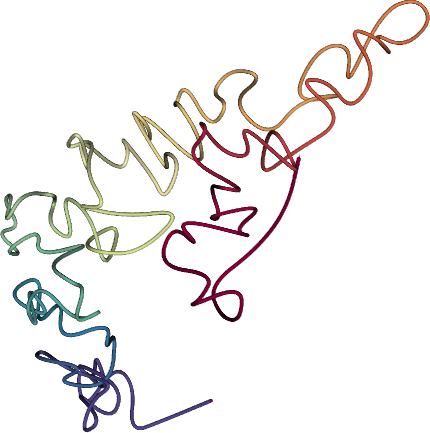
\includegraphics[width=0.5\linewidth]{images/yeast_chr2.png}
}
\begin{overlayarea}{0.9\linewidth}{2cm}
\only<5->{%
\vspace{1em}
\begin{flushright}
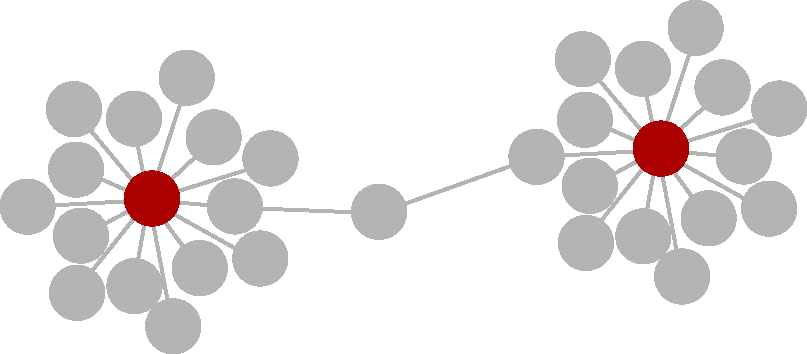
\includegraphics[width=0.8\linewidth]{figures/grn.pdf}
\end{flushright}
}
\end{overlayarea}
\end{column}
\end{columns}
\end{overlayarea}
\end{frame}


\begin{frame}
\frametitle{Analyse en médiation \& inférence causale}
\begin{figure}
\only<1>{%

\includegraphics[width=0.6\linewidth]{images/mediation_analysis.pdf}
}%
\only<2>{%
\includegraphics[width=0.6\linewidth]{images/mediation_analysis_direct.pdf}
}%
\only<3>{%
\includegraphics[width=0.6\linewidth]{images/mediation_analysis_indirect.pdf}
}%
\only<4->{%

\includegraphics[width=0.6\linewidth]{images/mediation_analysis_moderation_moderating.pdf}
}
\end{figure}
\vspace{1em}
{\bf \small L'analyse en médiation}
\vskip-1.3ex
\rule{\dimexpr\paperwidth-1.5cm\relax}{0.4pt}
\begin{itemize}
\footnotesize
\item<1->[-] Permet de distinguer les effets directs et indirects d'une variable
sur une autre.
\item<4->[-] Permet de trouver l'effet direct d'une variable sur une autre en présence d'un
garde-barrière.
\item<5->[-] Méthode reposant sur des tests d'hypothèses, développée pour des
données en basse dimension.
\item<6->[-] Regain d'intérêt dans la communauté informatique et statistique.
\end{itemize}
\end{frame}

\begin{frame}
\frametitle{Inférence causale pour les réseaux de régulation de gènes}
\begin{overlayarea}{12cm}{5.5cm}
\vspace{-0.5em}
\begin{figure}
\centering
\only<1>{%
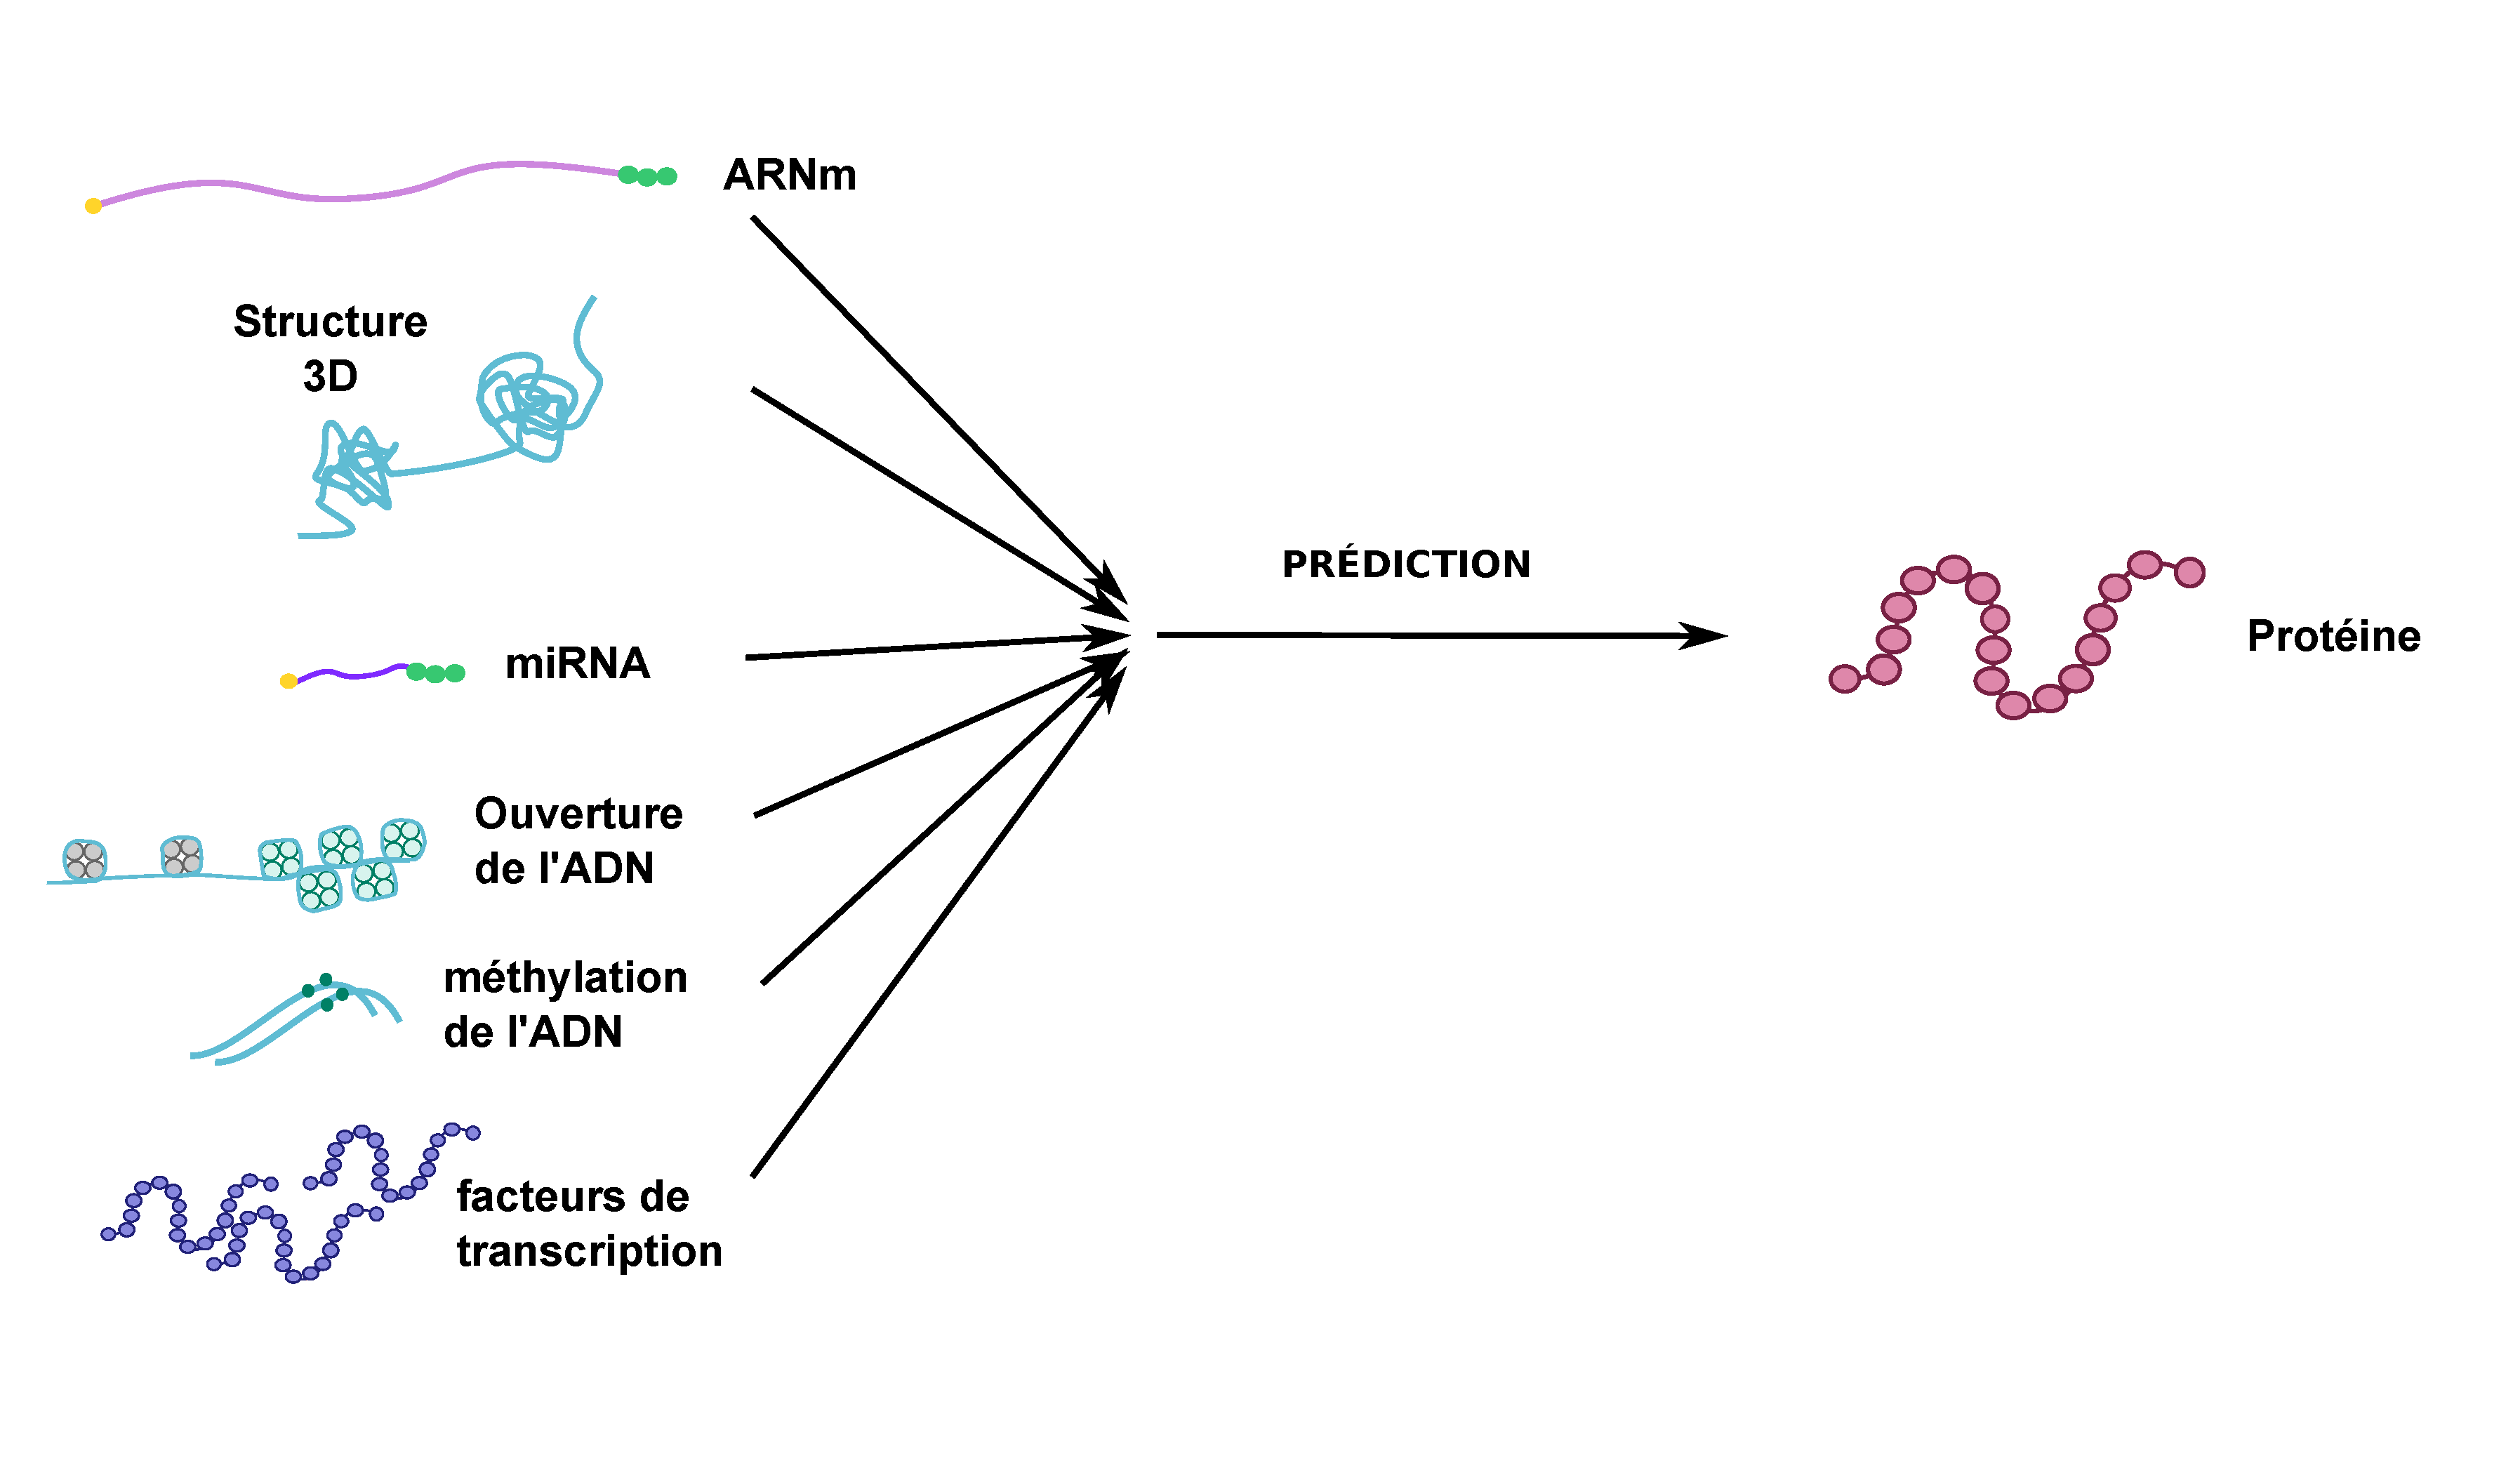
\includegraphics[width=0.8\linewidth]{schemas/donnees_epigenetiques.pdf}}
\only<2->{%
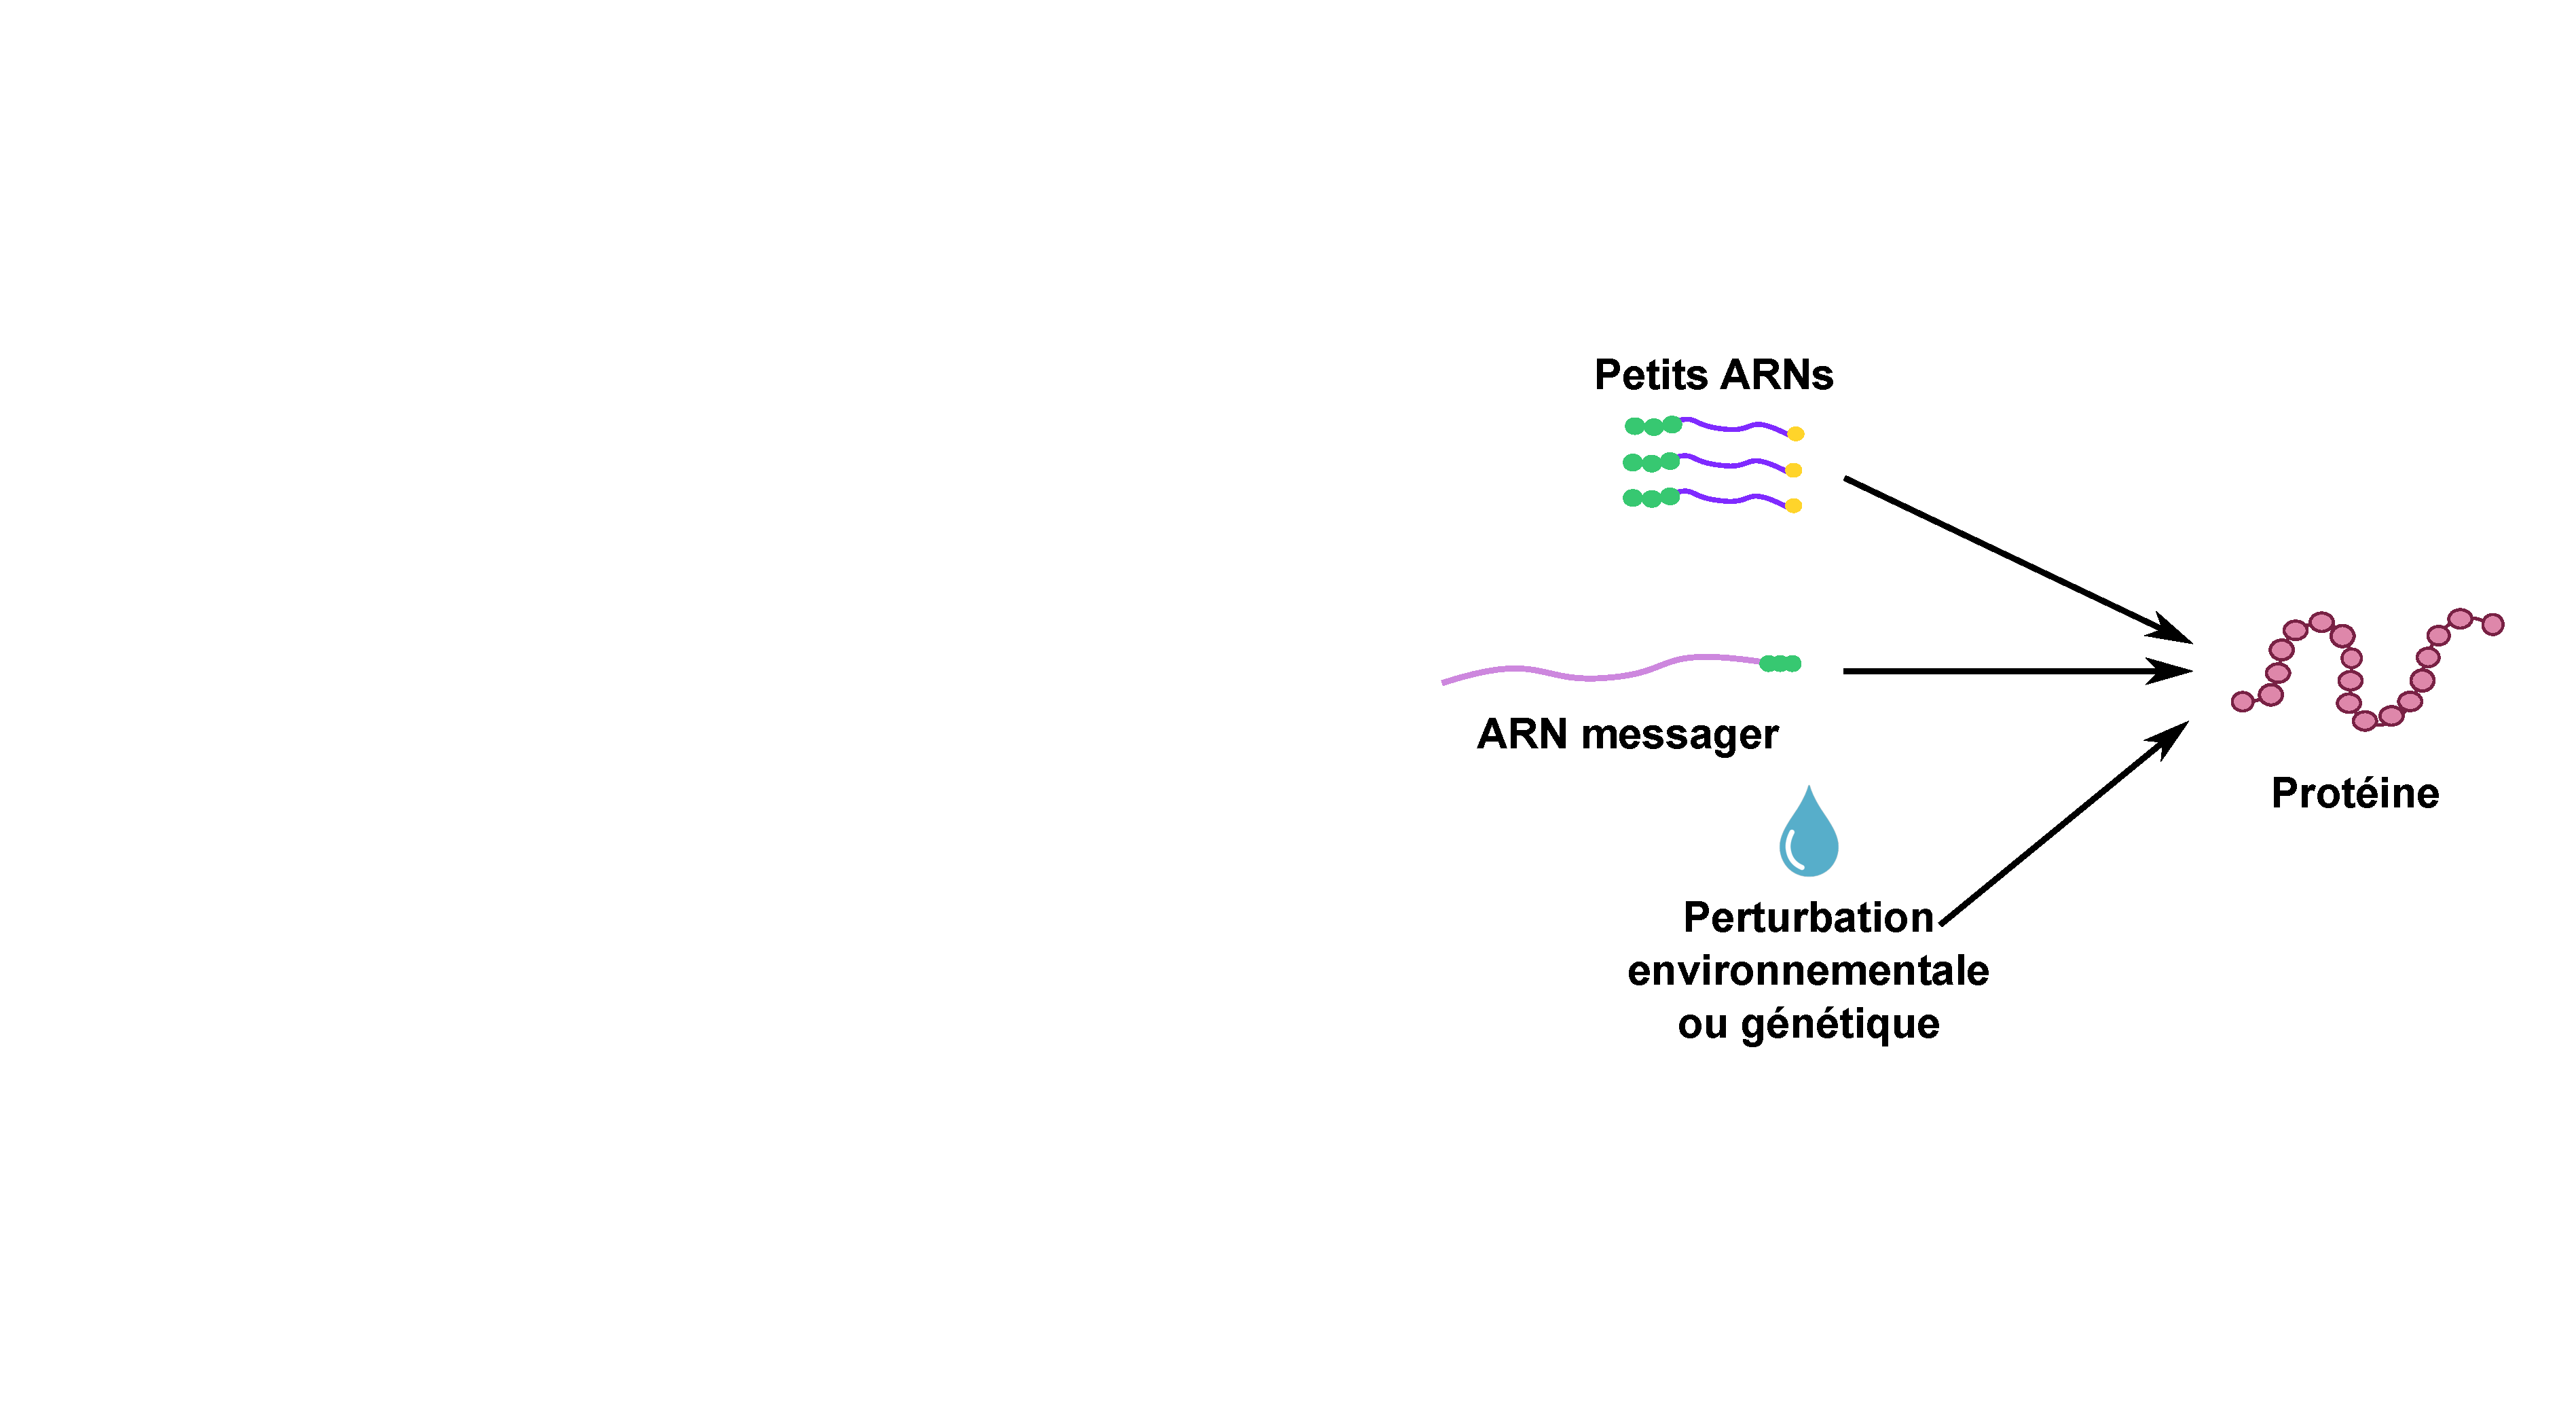
\includegraphics[width=0.8\linewidth]{schemas/analyse_en_mediation_final.pdf}}
\end{figure}
\end{overlayarea}

\vspace{-1em}
\begin{overlayarea}{12cm}{6cm}
\only<1>{{\bf \small Approche d'apprentissage statistique classique}}
\only<2->{{\bf \small L'analyse en médiation pour un gène}}
\vskip-1.3ex
\rule{\dimexpr\paperwidth-1.5cm\relax}{0.4pt}
\begin{columns}
\begin{column}{0.55\linewidth}
\only<1>{%
\begin{equation*}
y_\text{\tiny proteine} = f(X_\text{\tiny mRNA}, X_\text{\tiny miRNA}, X_\text{\tiny 3D},
X_\text{\tiny methyl}, X_\text{\tiny TF})
\end{equation*}
}
\only<2>{%
\begin{align*}
y_{\text{\tiny proteine}} &= \beta_{\text{\tiny mRNA}}X_{\text{\tiny mRNA}} + \beta_{\text{\tiny{miRNA}}}
X_{\text{\tiny{miRNA}}} \\
\end{align*}}
\only<3>{%
\begin{align*}
y_{\text{\tiny proteine}} &= \beta_{\text{\tiny mRNA}}X_{\text{\tiny mRNA}} + \beta_{\text{\tiny{miRNA}}}
X_{\text{\tiny{miRNA}}} \\
X^{\text{\tiny mRNA}} &=  f(X_{\text{\tiny methyl}}) g(X_\text{\tiny
3D})h(\beta_\text{\tiny
TF}X_{\text{\tiny TF}}) \\
\end{align*}}
\only<4->{%
\begin{align*}
y_{\text{\tiny proteine}} &= \beta_{\text{\tiny mRNA}}X_{\text{\tiny mRNA}} + \beta_{\text{\tiny{miRNA}}}
X_{\text{\tiny{miRNA}}} \\
X^{\text{\tiny mRNA}} &=  f(X_{\text{\tiny methyl}}) g(X_\text{\tiny
3D})h(\beta_\text{\tiny
TF}X_{\text{\tiny TF}}) \\
X^{\text{\tiny methyl}} &= \beta^\text{\tiny methyl}_\text{\tiny miRNA}
X_\text{\tiny miRNA}
\end{align*}
}
\end{column}
\begin{column}{0.45\linewidth}
\only<5->{%
{\bf \scriptsize Défis}
\vskip-1.3ex
\rule{\dimexpr\linewidth-.5cm\relax}{0.4pt}
\begin{itemize}[leftmargin=*]
\scriptsize
\item[-] Nombre de médiateurs potentiels élevé.
\item[-] Choix des descripteurs.
\item[-] Inférence non-paramétrique de la forme des fonctions modératrices.
\end{itemize}}
\end{column}
\end{columns}
\end{overlayarea}
\end{frame}

\begin{frame}
\frametitle{Inférence causale pour les réseaux de régulation de gènes}
\begin{overlayarea}{12cm}{5.5cm}
\vspace{-0.5em}
\begin{figure}
\centering
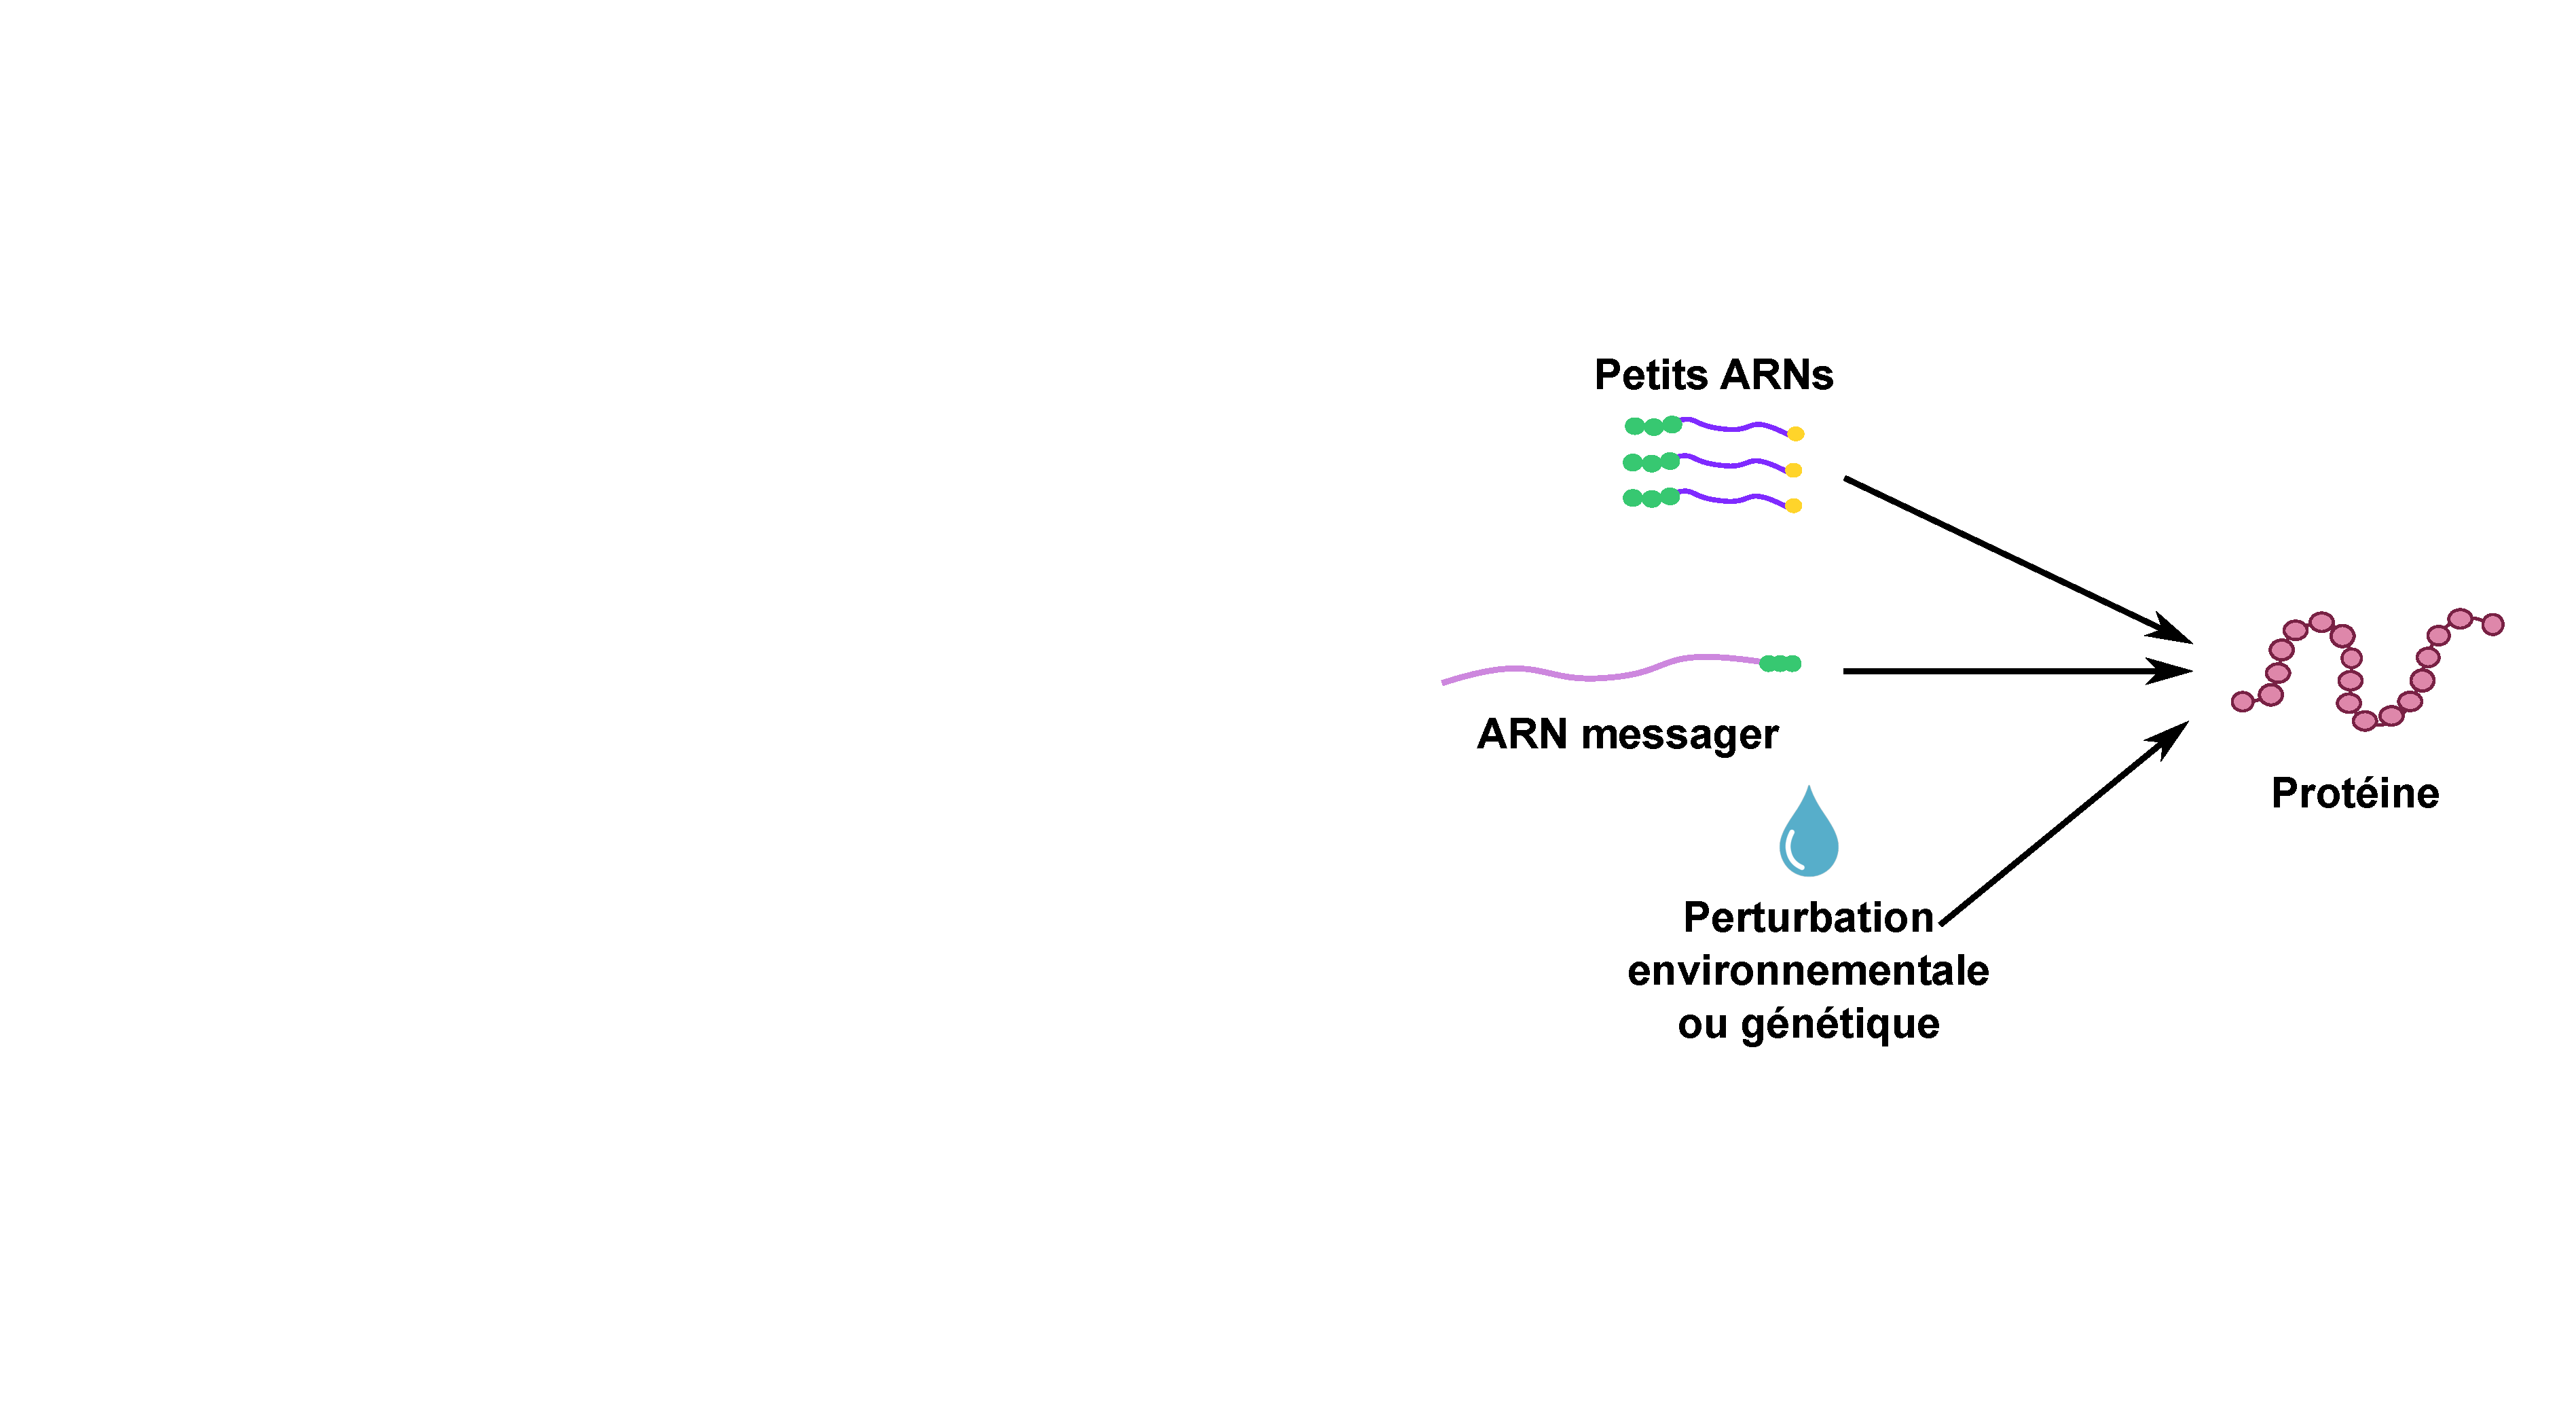
\includegraphics[width=0.8\linewidth]{schemas/analyse_en_mediation_final.pdf}
\end{figure}
\end{overlayarea}

\vspace{-1em}
\begin{overlayarea}{12cm}{6cm}
{\bf \small Mise à l'échelle au génome entier : multi-tâches et régularisation}
\vskip-1.3ex
\rule{\dimexpr\paperwidth-1.5cm\relax}{0.4pt}
\begin{itemize}
\footnotesize
\item[-] {\bf Défi :}\quad {\scriptsize 20~000 gènes chez la drosophile.}
\item[-] {\bf Stratégies proposées :}
\begin{itemize}
\scriptsize
\item[-] Augmenter le nombre d'échantillons via d'autres jeux de données.
\item[-] Partage de l'information entre gènes.
\end{itemize}
\item[-] {\bf Solutions :} \quad {\scriptsize Exploiter les approches
multi-tâches, d'inférence post-sélection, optimisation stochastique à grande
échelle}
\end{itemize}
\end{overlayarea}
\end{frame}


\begin{frame}
\frametitle{Résumé}
\begin{itemize}
\small
\item[-] Profil de recherche interdisciplinaire
\item[-] Programme de recherche \\
\begin{itemize}
\item Apprentissage statistique en haute dimension : structures,
régulations et fonction des génomes
\end{itemize}
\item[-] Recherche reproductible via des outils informatiques libres et
performants.
\item[-] Intégration au laboratoire d'accueil et l'écosystème local :
\end{itemize}

\begin{columns}
\begin{column}{0.49\linewidth}
\centering
\tiny
{\bf LIRIS -- UMR 5205}
\end{column}
\begin{column}{0.49\linewidth}
\tiny
\centering
{\bf Écosystème lyonnais}
\end{column}

\end{columns}
\begin{columns}
\tiny
\begin{column}{0.49\linewidth}
\begin{itemize}
\item[-] {\color{red} Équipe BEAGLE} (Biologie computationelle)
\item[-] Équipe DM2L (Apprentissage statistique)
\item[-] Équipe M2DISCO (Analyse géométrique et topologique)
\item[-] Équipe SICAL (Interaction \& collaboration)
\end{itemize}
\end{column}

\begin{column}{0.49\linewidth}
\begin{itemize}
\item[-] CIRC (World Health Organization)
\item[-] ICJ (UMR 5208)
\item[-] LBMC (UMR 5239)
\item[-] LBBE (UMR 5558)
\end{itemize}
\end{column}
\end{columns}

\vspace{1em}
{\bf \small Production scientifique}
\vskip-1.3ex
\rule{\dimexpr\paperwidth-1.5cm\relax}{0.4pt}
\begin{itemize}
\scriptsize
\item[-] 10 publications de rang A dont 5 premier auteur, 2 deuxième auteur.
Plus de 800 citations.
\item[-] 2 publications soumises, 6 en cours de rédaction
\item[-] Contributions majeures à 6 logiciels libres (dont
\texttt{scikit-learn}, \texttt{Matplotlib} et \texttt{scikit-image})
\end{itemize}
\end{frame}

\begin{frame}[t, noframenumbering]
\frametitle{Publications}

{\bf \small Publication de rang A, premier auteur}
\vskip-1.3ex
\rule{\dimexpr\paperwidth-1.5cm\relax}{0.4pt}
\begin{itemize}
\small
\item[-] Unfolding the Genome: The Case Study of {\em P. falciparum}. {\color{red}
Varoquaux} (2018)
\item[-] Effective normalization for copy number variation in Hi-C data.
Servant$^*$, {\color{red} Varoquaux$^*$} et al. (2018)
\item[-] Accurate identification of centromere locations in yeast genomes
using Hi-C. {\color{red} Varoquaux} et al. (2015)
\item[-] A statistical approach for inferring the 3D structure of the genome.
{\color{red} Varoquaux} (2014)
\item[-] Three-dimensional modeling of the P. falciparum genome during the
erythrocytic cycle reveals a strong connection between genome architecture and
gene expression. Ay, Bunnik, {\color{red} Varoquaux$^*$} et al. (2014)
\end{itemize}
\end{frame}

\begin{frame}[t, noframenumbering]
\frametitle{Publications}

{\bf \small Publication de rang A, deuxième auteur}
\vskip-1.3ex
\rule{\dimexpr\paperwidth-1.5cm\relax}{0.4pt}
\begin{itemize}
\small
\item[-] The Types, Roles, and Practices of Documentation in Data Analytics
Open Source Software Libraries. Geiger, {\color{red} Varoquaux} et al. (2018)
\item[-] HiC-Pro: an optimized and flexible pipeline for Hi-C data processing.
\quad Servant, {\color{red} Varoquaux} et al. (2015)
\end{itemize}

{\bf \small Autres publications de rang A}
\vskip-1.3ex
\rule{\dimexpr\paperwidth-1.5cm\relax}{0.4pt}
\begin{itemize}
\small
\item[-] Changes in genome organization of parasite-specific gene families
during the Plasmodium transmission stages. \quad Bunnik$^*$, Cook$^*$,
{\color{red} Varoquaux} et al. (2018)
\item[-] Identifying multi-locus chromatin contacts in human cells using
tethered multiple 3C. Ay, Vu, Zeitz, {\color{red} Varoquaux} (2015)
\item[-] A community effort to assess and improve drug sensitivity prediction
algorithms. Costello et al. (2014)
\end{itemize}
\end{frame}

\begin{frame}[t, noframenumbering]
\frametitle{Publications}
{\bf \small Autres publications}
\vskip-1.3ex
\rule{\dimexpr\paperwidth-1.5cm\relax}{0.4pt}
\begin{itemize}
\small
\item[-] Measuring cluster stability for bayesian non-parametrics using the
linear bootstrap
\item[-]
\end{itemize}

{\bf \small Publications soumises}
\vskip-1.3ex
\rule{\dimexpr\paperwidth-1.5cm\relax}{0.4pt}
\begin{itemize}
\item[-] Lifecycle transcriptomics of field-droughted sorghum reveals rapid
biotic and metabolic responses. \quad {\color{red} Varoquaux$^*$}, Cole$^*$,
Gao$^*$ et al. 
\item[-] FIXME pipeline paper
\item[-] JOSS
\end{itemize}

{\bf \small Publications en cours de rédaction}
\vskip-1.3ex
\rule{\dimexpr\paperwidth-1.5cm\relax}{0.4pt}
\begin{itemize}
\item[-] jupyter
\item[-] documentation
\item[-] FOSS with Alex
\item[-] Clustering
\item[-] NB structure
\item[-] Diploid
\end{itemize}
\end{frame}

\begin{frame}[t, noframenumbering]
\frametitle{}
\end{frame}

\end{document}

